\documentclass[12pt,a4paper]{report}

% File con pacchetti e impostazioni
% Caricamento pacchetti
\usepackage[utf8]{inputenc}
\usepackage[T1]{fontenc}
\usepackage[italian]{babel}
\usepackage{float}
\usepackage[hidelinks]{hyperref}
\usepackage{siunitx}
\usepackage[table]{xcolor}
\usepackage{array}
\usepackage{tabularx}
\usepackage{graphicx}
\usepackage[table]{xcolor} % nel preambolo

%Table of Contents
\usepackage{tocloft}
\renewcommand{\cftdot}{.}        % definisce il simbolo usato per i puntini
\renewcommand{\cftdotsep}{1}   % definisce la spaziatura tra i puntini

% Times New Roman (con matematica coerente)
\usepackage{newtxtext,newtxmath}

% Numerazione sezioni fino al terzo livello
\setcounter{secnumdepth}{3}

% Grafica e figure
\usepackage{graphicx}
\graphicspath{{immagini/}}

% Tabelle migliori
\usepackage{booktabs}

% Gestione citazioni
\usepackage{cite}

% Hyperlink
\usepackage{hyperref}
\hypersetup{
    colorlinks=true,
    linkcolor=blue,
    citecolor=blue,
    urlcolor=blue
}




\begin{document}



\tableofcontents


% Capitoli
\chapter{Introduzione}
\label{chap:introduzione}

\section{Contesto e limiti delle onde elettromagnetiche}
Le reti di sensori in ambienti sotterranei pongono sfide peculiari alla comunicazione wireless. 
La propagazione delle \emph{onde elettromagnetiche} nel sottosuolo soffre di attenuazioni elevate dovute alla 
permittività, alla conducibilità del terreno e all'umidità, con conseguente riduzione drastica della portata e 
dell'affidabilità dei link radio \citep{akyildiz2006}. 

Alcune soluzioni proposte in letteratura includono l'uso di frequenze super-high ed ultra-high (SHF, UHF) con l'obiettivo 
di implementare sistemi di tracking e monitoraggio in miniere di carbone, gallerie o condotti \citep{jacksha2016}.
Tuttavia, queste frequenze a causa della loro natura fisica sono soggette a forti perdite di segnale e riflessioni multipath,
limitando la copertura a range dai 10 ai 33 metri in condizioni ottimali con l'ausilio di antenne direzionali con un altezza 
pari a 1.2 metri l'una; questa tecnologia inoltre mostra tutta la sua vulnerabilità in presenza di curve strette (90°) o ostacoli.

\begin{figure}[H]
    \centering
    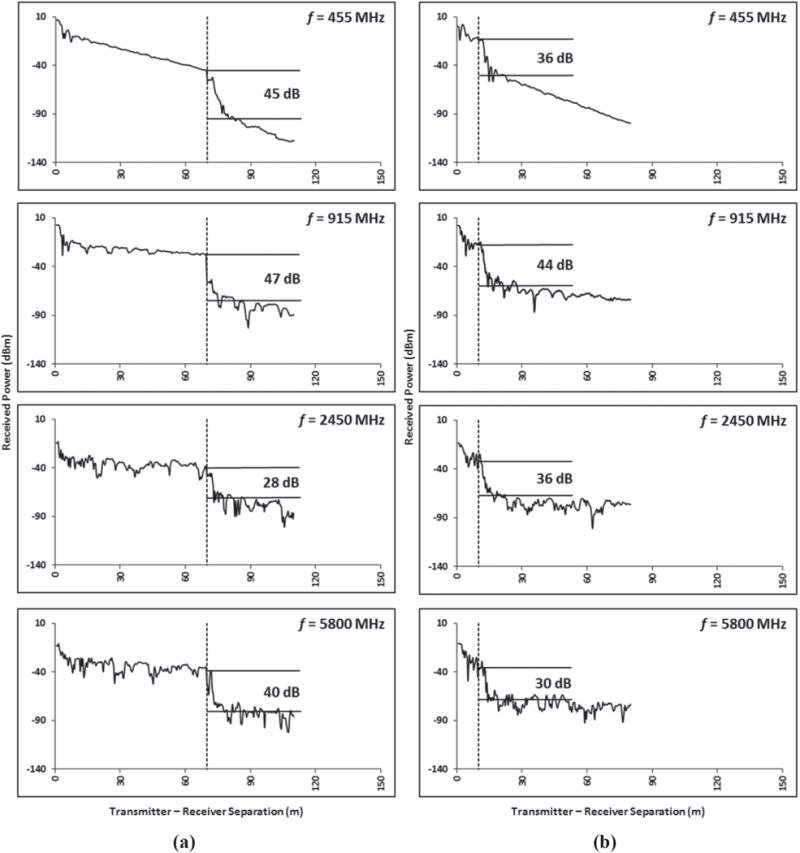
\includegraphics[width=0.35\textwidth]{immagini/corner_loss_em.jpg}
    \caption{Corner Loss \textasciitilde 30 dB in un condotto con angolo di 90° per radio frequenze HF/SHF \citep{jacksha2016}.}
    \label{fig:esempio}
\end{figure}

\section{Motivazione dell’approccio acustico}
Da questa problematica nasce la presente tesi, che si pone l’obiettivo di progettare e validare un 
\textbf{protocollo di comunicazione acustica} per reti \textbf{master--slave} in ambienti sotterranei, che dovrà essere: \textbf{efficiente, robusta ed economica}. 

L’idea è sfruttare la \emph{propagazione del suono nell’aria} presente in cavità, condotti o tunnel, trattando l’aria 
come un canale guida all'interno degli spazi confinati, e più in generale impiegare l’onda acustica come 
mezzo portante laddove il canale elettromagnetico è troppo penalizzato. 

\section{Richiami teorici sulla propagazione acustica}
In effetti, l’aria può essere modellata come un fluido compressibile: le variazioni locali di pressione e densità generate da una sorgente si propagano come onde longitudinali, 
la cui dinamica è descritta dall’equazione delle onde acustiche. 
La velocità di propagazione, che in condizioni standard 
è circa \SI{343}{m/s}, dipende da temperatura, pressione e composizione del gas, secondo la relazione 
$c = \sqrt{\gamma p_0 / \rho_0}$. 

Questa visione permette di trattare l’aria non solo come “spazio vuoto”, ma come un 
vero e proprio \emph{canale fisico}, caratterizzato da attenuazioni dovute a dispersione geometrica, assorbimento atmosferico 
e riverberi dovuti alle superfici \citep{Kinsler,MorseIngard,Pierce}. 

Il fine ultimo della rete sarà quello di permettere lo scambio di dati tra nodi utilizzando frequenze sonore sub-9kHz, appartenenti al range 1-10kHz: 
queste frequenze sono scelte per il loro compromesso tra portata e qualità del segnale \citep{Heifetz2017ANL}. 
L'applicazione principale è destinata al monitoraggio post-disastro, considerando che in altri contesti l'utilizzo di segnali acustici potrebbe risultare disturbante. 
I sensori saranno, inoltre, in grado di rilevare la presenza di corpi umani o gas tossici a seguito di crolli o esplosioni,
e trasmettere queste informazioni a un nodo master situato in superficie o in una zona sicura. 

\section{Motivazioni sperimentali e obiettivi della tesi}
La letteratura recente indica che, in scenari confinati, segnali acustici a bassa frequenza possono mantenere 
un rapporto segnale/rumore utilizzabile su distanze dell'ordine delle decine di metri, con modalità di propagazione 
\emph{lungo condotti} (ad esempio tubazioni o gallerie) e con modelli di attenuazione prevedibili 
\citep{acoustic2024}.  

Queste evidenze motivano la definizione di un protocollo leggero e robusto (rilevazione spettrale, soglie adattive con ausilio di machine learning) che faccia uso di componenti economici e facilmente integrabili (microfoni/codec, 
amplificatori, altoparlanti) per creare un \emph{layer fisico} acustico e il relativo \emph{protocollo di accesso}.

\section{Contributi attesi}
In sintesi, i contributi attesi sono: 
\begin{enumerate}
\item modellazione e scelta dei parametri del canale acustico in aria in ambienti confinati;
\item progettazione di un protocollo master--slave basato su pattern di frequenze, ACK e gestione del ritardo casuale;
\item implementazione hardware/software a basso costo;
\item validazione sperimentale mediante misure di SPL a diverse distanze, con stima dei livelli attesi per amplificazioni maggiori tramite traslazione dei valori rilevati.
\end{enumerate}

\chapter{Stato dell'Arte}
\label{chap:stato_arte}

\section{Tecnologie IoT}
L'Internet of Things (IoT) rappresenta una rete di dispositivi fisici, veicoli incorporati con elettronica, software, sensori e connettività di rete.
Questi dispositivi sono progettati per raccogliere e scambiare dati, consentodogli di comunicare con l'ambiente circostante.
Negli anni diverse tecnologie sono state usate per far comunicare questi dispositivi, la maggiorparte di queste si basano su radio frequenze, 
come LoRa, NB-IoT, ZigBee, Wi-Fi, BLE, fortemente indirizzate ad un uso outdoor o indoor. \\

Tuttavia, esistono scenari in cui la propagazione elettromagnetica incontra limiti
strutturali, ad esempio in ambienti sotterranei, gallerie, miniere o condotti, dove
l'attenuazione del segnale cresce a causa della composizione del terreno e
dell'umidità. In questi contesti, l'affidabilità della comunicazione wireless
tradizionale risulta fortemente compromessa.

\section{Comunicazione in ambienti sotterranei}
La comunicazione in ambienti sotterranei rappresenta una sfida significativa a causa delle caratteristiche uniche di questi ambienti.
Le onde elettromagnetiche, comunemente utilizzate per la comunicazione wireless, soffrono di attenuazioni elevate dovute alla permittività
del terreno e all'umidità, con una conseguente riduzione della portata e dell'affidabilità dei ponti radio \citep[sec.~2]{akyildiz2006}.\\
In letteratura è possibile individuare diverse soluzioni proposte per affrontare queste sfide, tra cui si riconoscono due linee principali di ricerca:
\begin{itemize}
    \item l'uso di radio frequenze molto basse (VLF), medie (MF)
          o più alte (UHF, SHF), adattate a condizioni specifiche;
    \item l'uso di onde acustiche, che sfruttano la propagazione meccanica del suono
          attraverso solidi e fluidi.
\end{itemize}
\subsection{Radio frequenze}
Le ricerche sulle onde elettromagnetiche in gallerie e miniere hanno mostrato
limiti significativi: la propagazione è fortemente influenzata dalla geometria degli
ambienti e dalle proprietà elettriche del mezzo.
Le ricerche effettuate sulle onde elettromagnetiche in gallerie e miniere 
mostrano limiti significativi riguardanti la propagazione, che risulta fortemente influenzata 
dalla geometria degli ambienti e dalle proprietà elettriche del mezzo.\\
Gli studi del U.S. National Institute for Occupational Safety and Health’s (NIOSH) Office of Mine Safety and Health Research (OMSHR)
\citep{jacksha2016}, avvenuti in seguito a crolli di alcune miniere di carbone
in U.S. nel 2006 hanno piantato le fondamenta per l'uso di one elettromagnetiche SHF/UHF in ambienti sotterranei.\\
Attraverso una serie di antenne direzionali dalla misura di 1.2 metri e ricevitori collocati prima in linea
retta ad una distanza crescente, e poi in presenza di curve a 30°, 60°, 90° e 180° in condotti sotterranei 
hanno dimostrato che, in condizioni ottimali, la copertura può raggiungere i 33 metri, ma la presenza di curve strette, biforcazioni
 o ostacoli riduce drasticamente la portata \citep[sec.~3]{jacksha2016};
 inoltre lo stesso fenomeno è stato osservato anche negli studi effettuati da Jeho Lee \citep[p.~59]{Lee2000_RadioWavePropagationTunnels}.

\begin{figure}[H]
    \centering
    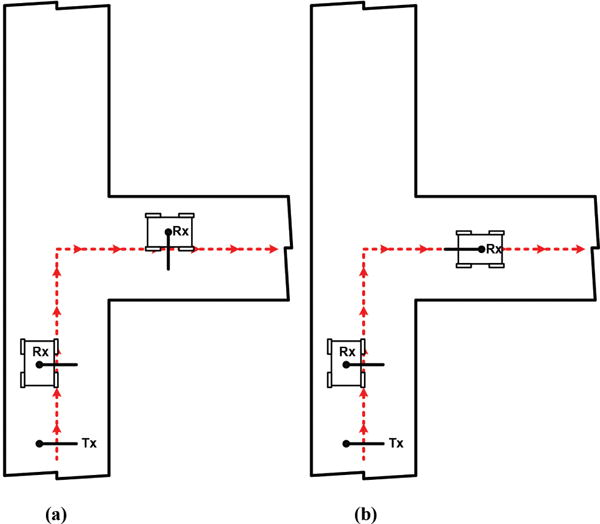
\includegraphics[width=0.30\textwidth]{immagini/corner_em.jpg}
    \caption{Mappa Tunnel U.S. National Institure for Occupational Safety and Health's\citep[sec.~3]{jacksha2016}.}
    \label{fig:esempio}
\end{figure}
Mentre
\citep[sec.~2]{akyildiz2006} descrivono le difficoltà intrinseche alla
propagazione sotterranea a causa di permittività e conducibilità elevate del terreno.\\

Più in generale, le tecnologie wireless pensate per ambienti sotterranei devono
fare i conti con una ridotta penetrazione delle frequenze tradizionalmente usate.\\
 Per questo, l'uso di frequenze estremamente basse (VLF, tra 3–30 kHz)
è stato studiato in scenari di emergenza e applicazioni militari, ma presenta
limiti di banda e di miniaturizzazione delle antenne \citep[sec.~5.1]{salam2023survey}.

\subsection{Onde acustiche}
Un'alternativa promettente alla comunicazione elettromagnetica in ambienti sotterranei è l'impiego di \emph{onde acustiche} (meccaniche), 
che si propagano attraverso solidi e fluidi (aria, acqua, fanghi di perforazione). A differenza delle onde EM, la propagazione acustica è 
spesso meno sensibile alla conducibilità elettrica del mezzo e può seguire percorsi guidati (ad es.\ lungo tubazioni o gallerie), con migliore 
resilienza a curve e biforcazioni \citep{fishta2023inpipe,heifetz2017pipes,farai2023mdpe}.

\paragraph{Modello di canale (cenni).}
Nei \textbf{solidi} (roccia, calcestruzzo, metalli, polimeri), la propagazione è dominata da onde elastiche (longitudinali e di taglio) e, in geometrie guidate 
(tubi, piastre, travi), da \emph{guided waves} (p.\,es.\ onde di Lamb o creep waves) con attenuazione che cresce fortemente con la frequenza e 
con il disaccoppiamento modale \citep[p.~2]{bianchi2023spazio}.\\ 
Nei \textbf{fluidi} in condotti (acqua/aria), il canale è tipicamente 
a bassa frequenza (centinaia di Hz–pochi kHz), con riflessioni multiple e dispersione; in vasche o condotti lunghi si osservano fenomeni di riverbero 
e frequenze di taglio dei modi guida \citep{fishta2023inpipe}. \\

\paragraph{Hardware e trasduttori.}
Sono impiegati trasduttori piezoelettrici o magnetostrittivi accoppiati meccanicamente al mezzo (collari su tubi, inserti su rocce/pareti, piastre di accoppiamento).\\
 Nei tubi metallici, coppie di attuatori/ricevitori permettono una comunicazione non invasiva (senza rompere il tubo), sfruttando onde di taglio o di Lamb 
 \citep[sec.~4.1]{heifetz2017pipes}.\\
Inoltre, per la comunicazione sotteranea si usano sorgenti e ricevitori acustici per mandare segnali nel terreno, 
fino a circa 50 m ma con velocità molto bassa (~20 bps) \cite[sec.~2.1]{yang2020soil}.\\

\paragraph{Tecniche di modulazione e codifica.}
Dato il canale fortemente dispersivo e soggetto a multi-percorso, si adottano modulazioni quali:
FSK/MFSK e BFSK a bassa frequenza creando collegamenti bassa velocità \citep{fishta2023inpipe,farai2023mdpe}.\\


\paragraph{Prestazioni riportate in letteratura.}
Risultati sperimentali rappresentativi includono:
\begin{itemize}
    \item \textbf{Suolo (through-soil).} Collegamenti fino a $\sim$50\,m con $\sim$20\,bps utilizzando portanti a bassa 
    frequenza e trasduttori compatti; dimostrazione di comunicazione digitale robusta in campi prova agricoli \citep[sec.~3]{yang2020soil}. 
    \item \textbf{Tubi metallici (acciaio).} Trasmissione di dati via onde elastiche lungo tubazioni esistenti in impianti industriali; 
    dimostrate immagini e pacchetti a centinaia di bps–pochi kbps su decine–centinaia di metri a bassa potenza, sfruttando onde di taglio
     e di Lamb \citep{heifetz2017pipes}.
    \item \textbf{Condotti idrici reali.} Revisione dei test in reti idriche urbane indica fattibilità di reti acustiche in-pipe per
     IoT, con vincoli di potenza, sincronizzazione e instradamento; lo stato dell’arte è pre-commerciale ma in rapida evoluzione \citep{fishta2023inpipe}.
\end{itemize}

\section{Applicazione della letteratura alla tesi}
La tesi si occuperà quindi della creazione di un protocollo di comunicazione acustica per sistemi distribuiti in ambienti sotteranei, 
basandosi sui risultati e le tecniche di cui sopra, è possibile quindi dedurre alcuni requisiti chiave:
Il protocollo opera nella banda 1–9 kHz, questa scelta è coerente con la letteratura, come visto nel \autoref{chap:introduzione}, 
inoltre l'utilizzo di una codifica FSK permetterà di avere un sistema robusto ma lento, coerentemente con le velocità di trasmissione viste in letteratura \citep{fishta2023inpipe}.\\

\chapter{Design del Protocollo}
\label{chap:design_protocollo}
\section{Architettura generale del sistema}
\begin{figure}[H]
    \centering
    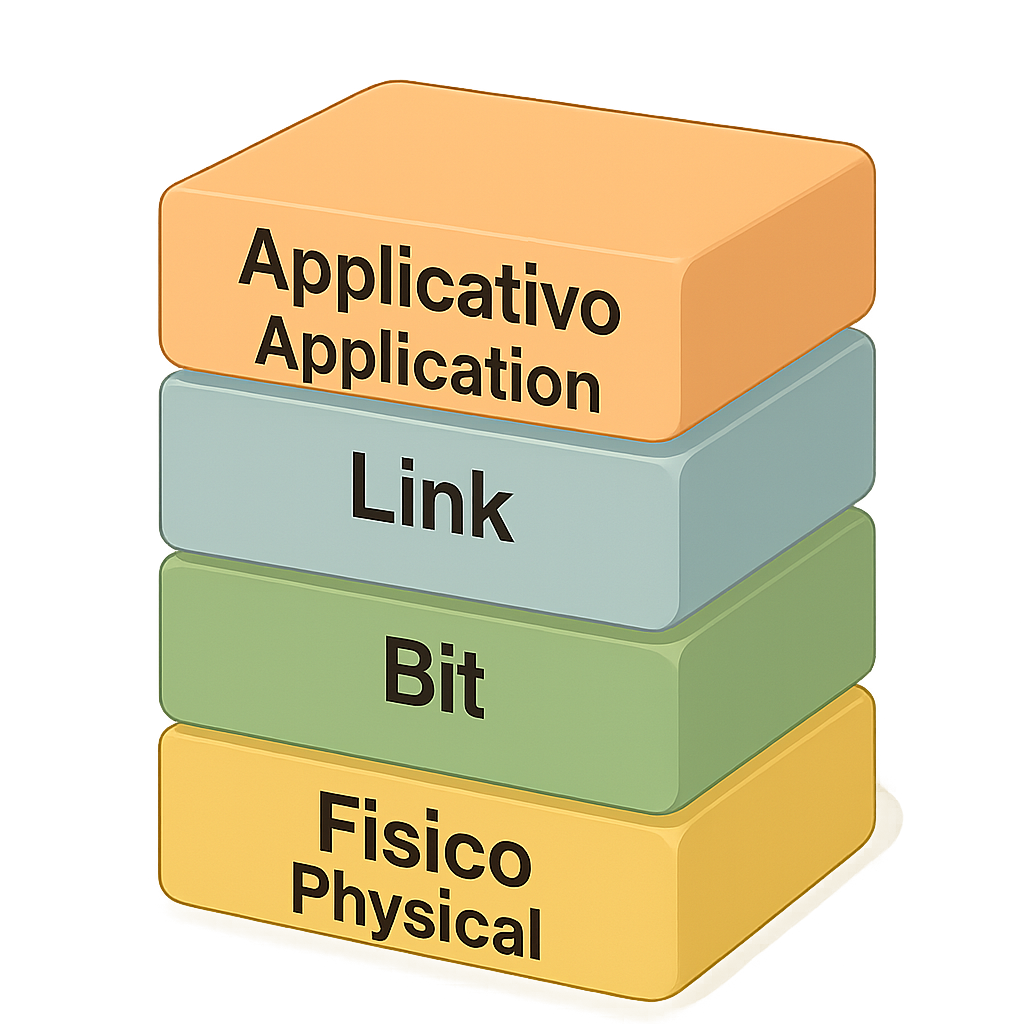
\includegraphics[width=0.35\textwidth]{immagini/layers.png}
    \caption{Livelli del Protocollo}
    \label{fig:esempio}
\end{figure}
Il protocollo è strutturaro in quattro livelli principali, ognuno con una funzione specifica.
\section{Livello Fisico}
Il livello fisico è responsabile della tramissione dei bit precedentemente composti dal livello Bit.
Questo sfrutta uno speaker per la trasmissione e un microfono per la ricezione dei bit che vengono trasmessi mediante coppie superimposte di frequenze.
\subsection{Ingresso}
Il microfono I2S è collegato al microcontrollore ESP32 tramite il bus I2S, sfruttando uno dei due canali disponibili.  
Il segnale audio viene campionato a $48\,\text{kHz}$ con una risoluzione di 16 bit, per poi essere gestito mediante due array in swapping, concetto che verrà approfondito successivamente. \\

\noindent
La scelta della frequenza di campionamento deriva dal \textbf{teorema di Nyquist-Shannon} \cite{shannon1949}, secondo il quale un segnale può essere ricostruito senza ambiguità se la frequenza di campionamento $f_s$ è almeno doppia rispetto alla massima frequenza del segnale $f_{\max}$:
\[
f_s \geq 2 f_{\max}.
\]
Ne consegue che la massima frequenza rappresentabile è
\[
f_{\text{Nyquist}} = \frac{f_s}{2}.
\]

Nel nostro caso:
\[
f_s = 48\,\text{kHz} \quad \Rightarrow \quad f_{\text{Nyquist}} = 24\,\text{kHz}.
\]

Poiché l’orecchio umano percepisce frequenze fino a circa $20\,\text{kHz}$ \cite{zwicker1999psychoacoustics}, la scelta di $48\,\text{kHz}$ garantisce la copertura dell’intero spettro udibile, con un margine di sicurezza di $4\,\text{kHz}$. Frequenze prossime al limite teorico di Nyquist risulterebbero invece difficili da catturare senza aliasing, a causa dei limiti pratici dei filtri anti-alias. \\

\noindent
Per l’elaborazione, i campioni vengono raccolti in blocchi di lunghezza $N = 512$. Con la frequenza di campionamento fissata:
\[
T_{\text{blocco}} = \frac{N}{f_s} = \frac{512}{48 \cdot 10^3} \approx 0.01066\,\text{s}.
\]
Ogni blocco di dati rappresenta quindi un intervallo di circa $10.7\,\text{ms}$ di segnale audio.  

\noindent
Una volta acquisito il blocco, viene calcolata la \textbf{trasformata veloce di Fourier (FFT)} \cite{cooley1965fft} per analizzare lo spettro in frequenza. La complessità della FFT cresce come $N \log_2 N$, e per $N=512$ si hanno circa:
\[
512 \cdot \log_2(512) = 512 \cdot 9 = 4608
\]
operazioni complesse.  

Sul microcontrollore ESP32 \cite{esp32techref}, operante a $120\,\text{MHz}$, questo si traduce in un tempo di elaborazione di circa $0.42\,\text{ms}$ per blocco, ovvero $\sim 0.83\,\mu\text{s}$ per campione. In termini di carico computazionale: $\sim 20$ moltiplicazioni, $\sim 29$ addizioni/sottrazioni e un’operazione di radice quadrata per campione, pari a $\sim 99$ cicli di clock.  

\noindent
Questo significa che, a fronte di una finestra temporale di $10.7\,\text{ms}$, l’FFT viene calcolata in meno del $5\%$ del tempo disponibile, consentendo un’elaborazione in tempo reale anche senza multi-threading.

\begin{figure}[H]
    \centering
    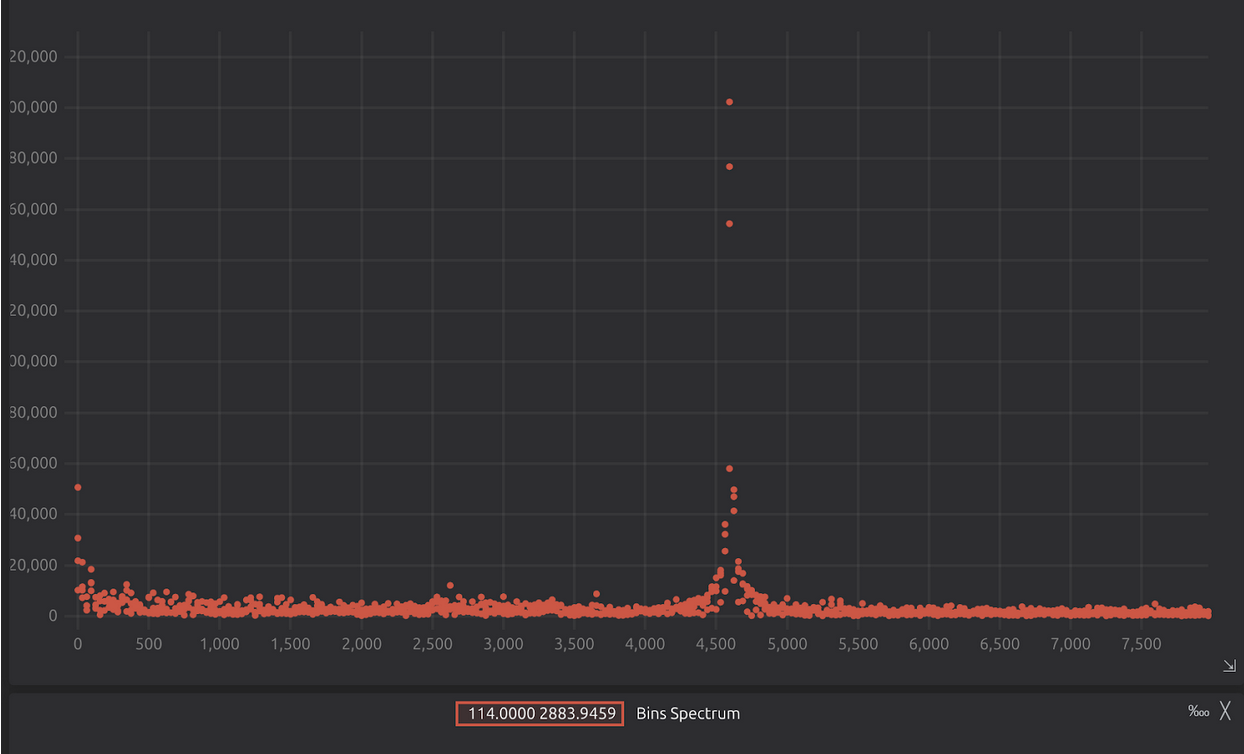
\includegraphics[width=0.9\textwidth]{immagini/fft_spectrum.png}
    \caption{Diagramma contentente lo spettro di frequenza calcolato tramite FFT} su un blocco di $512$ campioni acquisiti a $48\,\text{kHz}$.
    \label{fig:spettro}
\end{figure}

Come da Fig.~\ref{fig:spettro}, si può osservare che lo spettro di frequenza ottenuto dalla FFT mostra picchi alle frequenze di interesse, ma mostra anche un rumore di fondo.
Durante la creazione di questo protocollo sono emerse diverse difficoltà legate alla presenza di rumore ambientale,
questa condizione ha reso necessario l'uso di tecniche di filtraggio.
\subsection{Filtraggio}
L'idea iniziale, quando il protocollo era ancora nelle prime fasi di vita, era quella di utilizzare una semplice soglia fissa (filtro passa-basso) per discriminare i picchi dal rumore.
Tuttavia, questa soluzione si è rivelata inefficace, in quanto i microfoni presentano una risposta in frequenza che cala sulle alte, quindi i livelli in dB delle frequenze alte risultavano attenuati, non facendogli superare la soglia passa basso.
Inoltre, il rumore ambientale non è costante, ma varia nel tempo e nello spettro, rendendo difficile stabilire una soglia fissa che funzioni in tutte le condizioni.\\ 
Successivamente si è pensato di utilizzare delle soglie fisse, che variassero per ogni frequenza, in modo da tenere conto della risposta in frequenza del microfono.
Al fine di calcolare queste soglie, è stato utilizzato un algoritmo di \textit{regressione lineare} per stimare la retta che meglio approssima l'andamento della soglia minima:
\[
y = \beta_{} + \beta_{}x + \varepsilon \rightarrow y = -301.751324 \times x + 48531.689491
\]
Dove x rappresenta il numero del Bin.

\include{capitoli/requisiti}
\chapter{Implementazione Hardware}
\label{chap:implementazione_hardware}
\section{Tecnologie di base}

In questo capitolo tratteremo tutte le tecnologie utilizzate nel progetto, come i microcontrollori e i dispositivi di output,
 concentrandoci sull’ESP32.

\subsection{Panoramica dell’ESP32}

\subsubsection{Generalità}
I microcontrollori (MCU) sono circuiti integrati che combinano nello stesso chip un microprocessore con una serie di componenti periferici
 come: memoria, timer, convertitori analogico-digitali e soprattutto pin di I/O.

A differenza di un microprocessore (CPU), i microcontrollori non sono pensati per svolgere onerose attività di calcolo ma per interagire 
il più possibile con l’ambiente esterno, gestendo numerosi scambi fra le periferiche di Input/Output.

L’ESP32, sviluppato da Espressif Systems, rappresenta un microcontrollore avanzato con architettura dual-core Tensilica LX6 a 32 bit
 (alcune varianti hanno anche core single-core o LX7), integrando al suo interno Wi-Fi e Bluetooth a basso consumo. Questa caratteristica
  lo rende particolarmente adatto per applicazioni IoT (Internet of Things), domotica e sistemi embedded complessi (Espressif, 2024 \cite{Espressif2024}).

\subsubsection{Famiglie di ESP32}
I microcontrollori sono suddivisi in famiglie a seconda del processore e delle periferiche integrate. Nel caso dell’ESP32,
 troviamo diverse varianti come ESP32-WROOM-32, ESP32-WROVER, ESP32-C3, ESP32-S2 ed ESP32-S3.  
Queste versioni condividono la stessa architettura di base ma differiscono per risorse di memoria, numero di GPIO disponibili,
 supporto a periferiche aggiuntive o funzionalità avanzate come acceleratori AI.  

La scelta del modulo da utilizzare deve essere fatta non sulla base delle prestazioni massime, ma dell’ottimalità rispetto al
 progetto in questione (Patti, 2024 \cite{Patti2024}).

\subsubsection{Componenti hardware}
Ogni ESP32 integra al suo interno non solo la CPU, ma anche le memorie e una grande quantità di periferiche digitali e analogiche, 
oltre ai moduli di comunicazione wireless (Wi-Fi 802.11 b/g/n e Bluetooth 4.2/5.0).  
Questa elevata integrazione consente di ridurre i costi, semplificare il design e garantire maggiore velocità di accesso ai dati.

\begin{figure}[H]
\centering
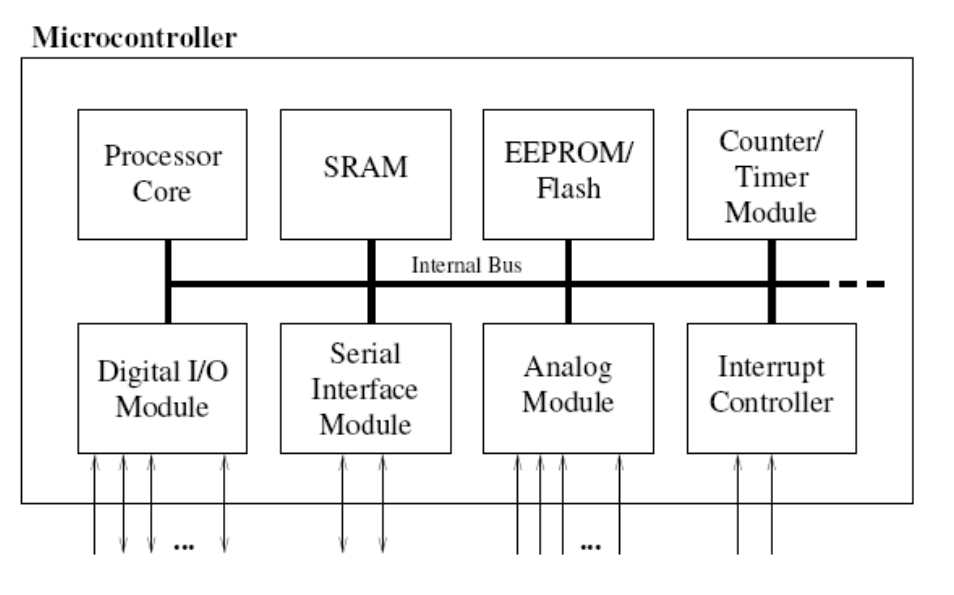
\includegraphics[width=0.7\textwidth]{esp32_block_diagram.png}
\caption{Componenti hardware principali di un microcontrollore ESP32.}
\label{fig:esp32-mcu}
\end{figure}

\subsubsection{Memorie}
Le memorie di un microcontrollore possono essere di tipo volatile e non volatile. Le volatili includono SRAM e DRAM; le non volatili comprendono ROM, EEPROM, Flash e, in alcuni casi, NVRAM.

L’ESP32 tipicamente dispone di:
\begin{itemize}
    \item 448 KB di ROM, che contiene il bootloader e alcune librerie di base;
    \item 520 KB di SRAM interna, divisa tra cache, stack e heap per le applicazioni;
    \item Flash esterna fino a 16 MB (a seconda del modulo), utilizzata per memorizzare codice e file system;
    \item opzionalmente, PSRAM esterna fino a 8 MB, utile per applicazioni che richiedono elaborazioni multimediali o server web embedded.
\end{itemize}

Rispetto ad altre schede, l’ESP32 si distingue per la disponibilità di memoria e per la presenza di connettività wireless integrata, rendendolo una soluzione più completa per progetti IoT e sistemi embedded avanzati (Patti, 2024 \cite{Patti2024}; Espressif, 2024 \cite{Espressif2024}).

\subsection{Periferiche di Input/Output}
Le periferiche di Input/Output (I/O) sono componenti essenziali che permettono al microcontrollore di interagire con il mondo esterno.
Per la realizzazione del progetto sono state utilizzate diverse periferiche, in questa sezione se ne approfondiscono le loro caratteristiche.\\
\noindent
Tutta la componentistica impiegata in questo progetto è stata selezionata dal catalogo \textbf{Adafruit Industries}. 
La scelta è motivata dall'elevata qualità dei loro moduli, dalla cura del layout dei circuiti stampati e dalla ricca documentazione tecnica a corredo, che garantiscono affidabilità in fase di prototipazione e semplicità di integrazione. 
L'utilizzo di componenti a marchio Adafruit riduce i rischi di incompatibilità o malfunzionamenti tipici dei cloni economici e assicura un supporto didattico di livello professionale.


\subsubsection{Microfono MEMS I2S digitale Adafruit -- SPH0645LM4H}
\label{subsec:mic}
Il breakout Adafruit (cod. 3421) monta il microfono MEMS digitale \textbf{Knowles SPH0645LM4H-B}, bottom–port, con uscita \textbf{I$^2$S} \cite{adafruit-guide,adafruit-product}. 
È un dispositivo \emph{slave} che richiede dal master le linee di clock (\texttt{BCLK}, \texttt{LRCLK}) \cite{nordic-devzone}. 
Fornisce direttamente campioni PCM a 24 bit (con 18 bit effettivi), evitando stadi analogici esterni \cite{knowles-datasheet}.
\begin{figure}[H]
  \centering
  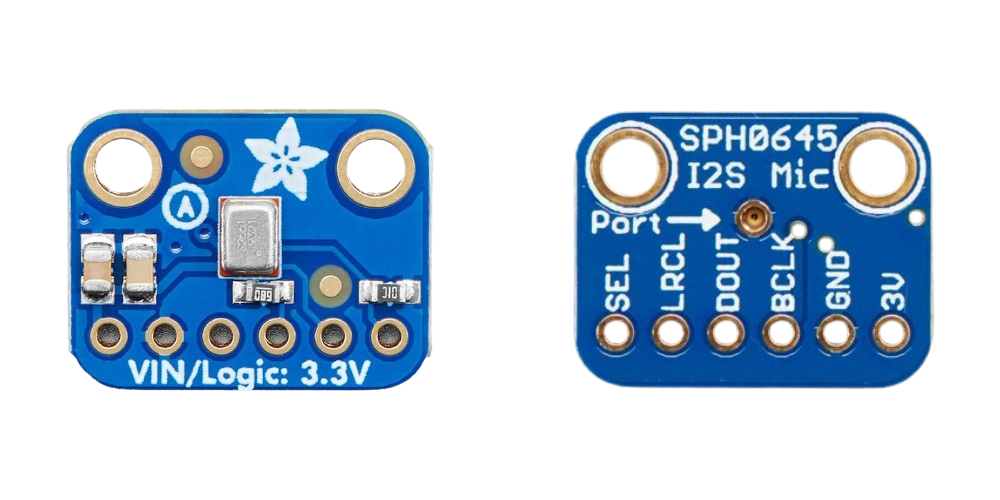
\includegraphics[width=0.7\textwidth]{adafruit_mems.png}
  \caption{Microfono MEMS I2S digitale Adafruit SPH0645LM4H-B.}
  \label{fig:adafruit_mems}
  \end{figure}

\paragraph{Caratteristiche principali.}
\begin{itemize}
  \item Alimentazione: \SIrange{1.62}{3.6}{V}, logica \SI{3.3}{V}, tipico consumo \SI{600}{\micro A} \cite{digikey-sheet}.
  \item Interfaccia: I$^2$S, pin \texttt{BCLK}, \texttt{LRCLK}, \texttt{DOUT}, \texttt{SEL}, più \texttt{3V} e \texttt{GND}.
  \item Formato dati: parole a 24 bit (MSB first, complemento a due), 18 bit utili, oversampling ratio (OSR) = 64 \cite{knowles-datasheet}.
  \item Prestazioni: SNR tip. \SI{65}{dB(A)}, AOP \SI{120}{dB\,SPL}, sensibilità $\sim -26$ dBFS @ \SI{94}{dB\,SPL} \cite{knowles-datasheet}.
\end{itemize}

\paragraph{Pinout e collegamenti.} 
Due moduli possono essere usati in stereo condividendo \texttt{BCLK}, \texttt{LRCLK}, \texttt{DOUT}; \texttt{SEL} basso/alto definisce L/R. 
In modalità mono basta un solo modulo con \texttt{SEL} a GND (Left di default) \cite{adafruit-guide}.

\paragraph{Interfaccia I$^2$S.} 
Il microfono trasmette in formato \emph{Philips}: ogni semiperiodo di \texttt{LRCLK} contiene una parola da 24 bit. 
La relazione fondamentale è $\mathrm{BCLK}=64f_s$ \cite{nordic-devzone}. 
Tipici: \SI{3.072}{MHz} per \SI{48}{kHz}, \SI{2.8224}{MHz} per \SI{44.1}{kHz}.

\paragraph{Catena del segnale interna.}
\begin{enumerate}
  \item Trasduttore MEMS capacitivo: diaframma + backplate $\to$ capacità $C(t)$.
  \item Amplificatore a carica: traduce $\Delta C$ in tensione.
  \item Modulatore $\Sigma\Delta$: noise–shaping fuori banda audio.
  \item Filtro di decimazione: riduce a $f_s$ mantenendo 18 bit effettivi.
  \item Serializer: prepara le parole I$^2$S.
\end{enumerate}

\paragraph{Fondamenti fisici.}
La pressione $p(t)$ agisce sul diaframma (massa $m$, molla $k$, smorzamento $b$) \cite{mems-acoustics}:
\[
m\ddot{x}+b\dot{x}+kx=S\,p(t)
\]
La variazione di capacità è $\Delta C/C_0 \approx x/d_0$, con risonanza a $\omega_0=\sqrt{k/m}$. 
Il rumore complessivo deriva da contributi termico–meccanici, elettronici e quantizzazione. 
Il back–volume e la porta acustica modellano la risposta in frequenza (roll–off alle basse, ondulazioni agli alti) \cite{mems-acoustics}.
\begin{figure}[H]
  \centering
  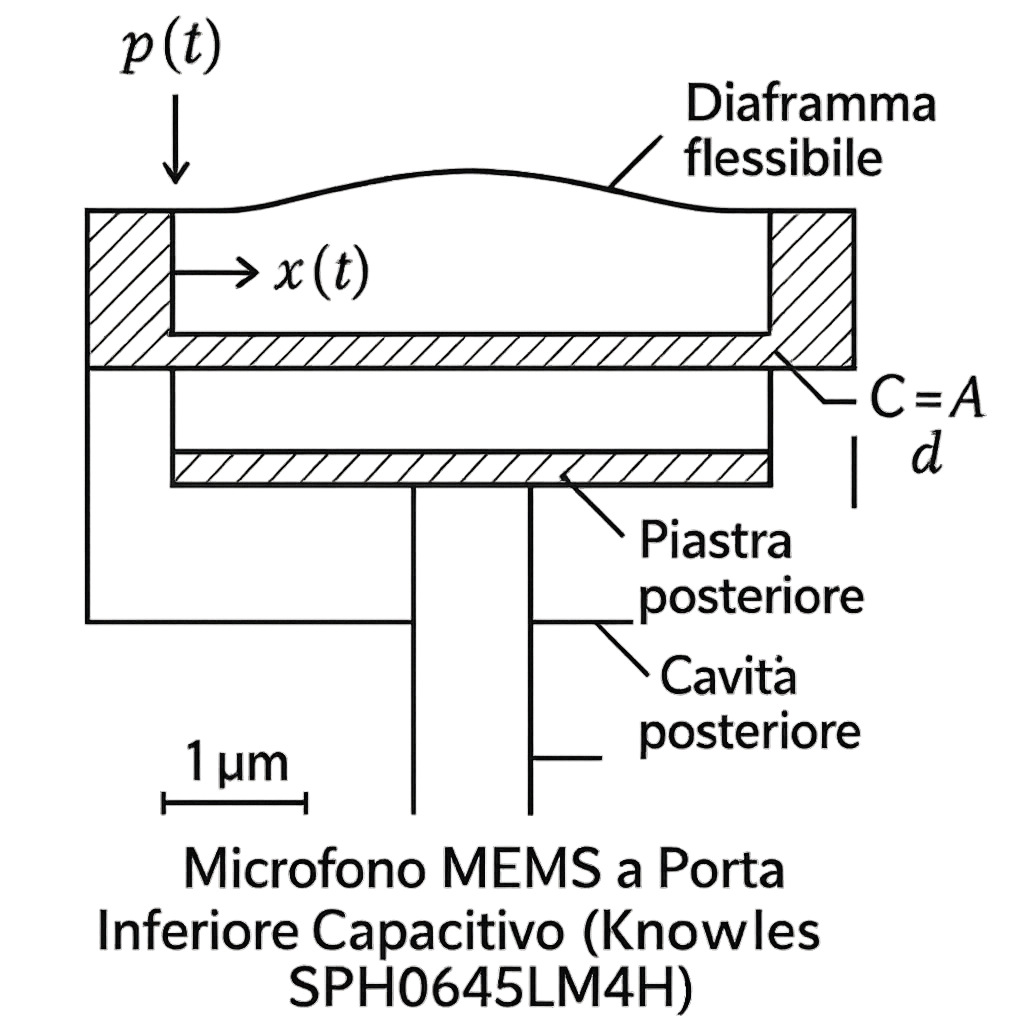
\includegraphics[width=0.4\textwidth]{adafruit_diaframma.png}
  \caption{Sezione verticale del microfono Adafruit MEMS.}
  \label{fig:adafruit_diaframma}
  \end{figure}

\paragraph{Limiti.} Non tollera \SI{5}{V}, banda garantita $\sim$\SI{20}{Hz}--\SI{10}{kHz} (utilizzabile fino a $\sim$\SI{15}{kHz} secondo Adafruit) \cite{adafruit-product}, OSR fisso (meno flessibile di PDM).

\paragraph{Relazione dBFS--SPL.}
\SI{94}{dB\,SPL} = \SI{1}{Pa} $\Rightarrow$ $\approx -26$ dBFS RMS \cite{knowles-datasheet}. 
L’AOP a \SI{120}{dB\,SPL} ($\sim$\SI{20}{Pa}) indica il massimo senza distorsione significativa.


\subsubsection{Adafruit MAX98357A I$^2$S Amplificatore Classe-D}

Il breakout Adafruit basato sul chip \textbf{MAX98357A} è un amplificatore audio digitale in classe D, in grado di convertire direttamente un flusso
 I$^2$S in segnale audio analogico amplificato per pilotare altoparlanti a bassa impedenza. 
La caratteristica principale è l’eliminazione della necessità di un DAC esterno: il MAX98357A integra al suo interno la conversione digitale-analogica, 
il filtraggio, e la sezione di potenza \cite{maxim-datasheet,adafruit-guide-max98357}.
\begin{figure}[H]
  \centering
  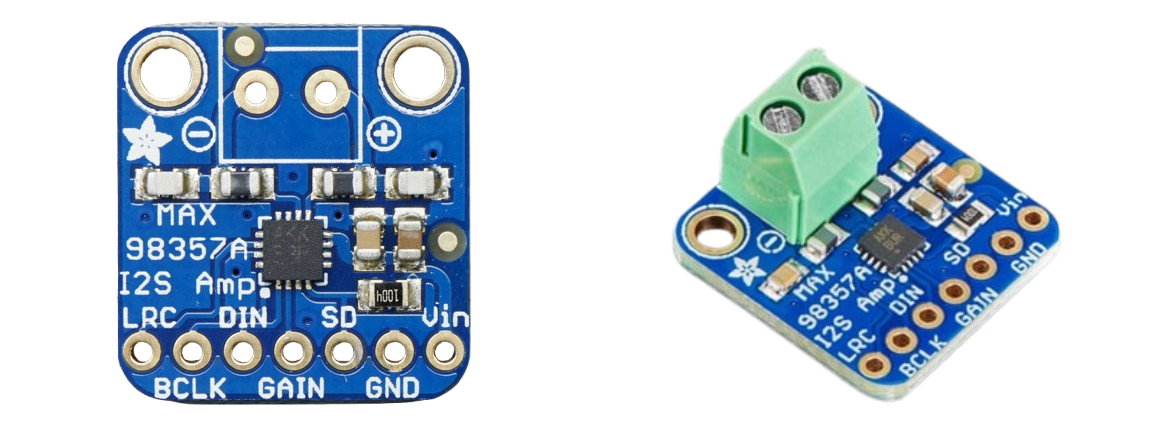
\includegraphics[width=0.7\textwidth]{adafruit_max.png}
  \caption{Amplificatore digitale Classe-D Adafruit MAX98357A.}
  \label{fig:adafruit_max}
  \end{figure}
\paragraph{Caratteristiche essenziali.}
\begin{itemize}
  \item \textbf{Alimentazione}: \SIrange{2.5}{5.5}{V}, con tensione tipica \SI{3.3}{V} o \SI{5}{V}. 
  \item \textbf{Potenza d’uscita}: fino a \SI{3.2}{W} su \SI{4}{\ohm} a \SI{5}{V}, THD+N $\approx$ \SI{1}{\%}.
  \item \textbf{Interfaccia}: I$^2$S standard (\texttt{BCLK}, \texttt{LRCLK}, \texttt{DIN}); pin aggiuntivi per modalità (\texttt{GAIN}, \texttt{SD}, \texttt{DMP}).
  \item \textbf{Efficienza}: superiore all’$\SI{85}{\%}$ grazie all’architettura in classe D.
  \item \textbf{Gamma dinamica}: $\approx \SI{98}{dB}$, con rumore di fondo contenuto \cite{maxim-datasheet}.
\end{itemize}

\paragraph{Funzionamento.}
Il MAX98357A riceve un flusso I$^2$S in formato PCM (\SI{16}{}, \SI{24}{} o \SI{32}{bit}, standard Philips). L’architettura interna comprende:
\begin{enumerate}
  \item \textbf{Interfaccia I$^2$S}: decodifica il flusso digitale e gestisce il framing (left/right).
  \item \textbf{DAC sigma–delta}: converte i campioni PCM in una modulazione a densità di impulsi.
  \item \textbf{Driver in classe D}: due MOSFET push-pull pilotano direttamente l’altoparlante in configurazione \emph{bridge-tied load (BTL)}.
  \item \textbf{Filtro LC virtuale}: la stessa induttanza del carico acustico e la risposta del driver fungono da filtro passa-basso, eliminando la componente PWM ad alta frequenza.
\end{enumerate}
\begin{figure}[H]
  \centering
  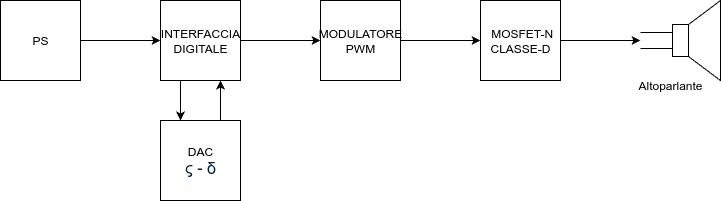
\includegraphics[width=0.7\textwidth]{max_diagram.png}
  \caption{Funzionamento interno del MAX98357A.}
  \label{fig:max_diagram}
  \end{figure}
\paragraph{Motivazioni fisiche del funzionamento.}
L’amplificatore in classe D si basa su modulazione a \emph{duty cycle} dei MOSFET: il segnale analogico ricostruito corrisponde al valore medio del PWM. L’elevata efficienza deriva dal fatto che i transistor lavorano quasi sempre in saturazione o interdizione, riducendo le perdite per dissipazione. L’integrazione del DAC sigma–delta consente un noise-shaping che sposta il rumore di quantizzazione fuori banda audio, garantendo un’ottima qualità percepita \cite{texas-classd}.

\section{Progettazione digitale}
Per la progettazione digitale del sistema è stato utilizzato il software \textbf{Fritzing}, un tool open-source
per la progettazione di circuiti elettronici, con la possibilità di creare moduli personaizzati.\\
Nel capito \ref{chap:design_protocollo} è stato descritto il protocollo di comunicazione, facendo riferimento al \textbf{Livello Fisico},
come il livello più basso del modello. L'interazione I/O con il mondo circostante che avviene nel Livello Fisico, è realizzata con due componenti: una software, 
che tratteremo a breve nel capitolo \ref{chap:implementazione_software}, e una hardware, che vedremo in questo capitolo.\\
Il Livello Fisico è realizzato con due periferiche di Input/Output, il microfono MEMS digitale e l'amplificatore Classe-D, che comunicano con il microcontrollore ESP32
 tramite il protocollo I$^2$S.\\

Per la realizzazione del circuito elettronico sono stati utilizzati due breakout board Adafruit, che integrano i componenti necessari per il corretto funzionamento
  del microfono e dell'amplificatore.\\
  L'utilizzo del microfono MEMS I2S digitale Adafruit SPH0645LM4H viene da una selezione accurata, basata su test di qualità,
  il progetto, che all'inizio prevedeva un microfono analogico, è stato modificato per utilizzare un microfono digitale,
  in quanto i test effettuati con il microfono analogico non hanno dato risultati soddisfacenti.\\



  \subsection{Collegamento del microfono digitale I$^2$S}
  \label{subsec:conn_mic}
  
  La \autoref{fig:board_microfono} mostra lo schema di cablaggio realizzato in \textbf{Fritzing} tra la breakout Adafruit basata sul microfono MEMS digitale \textbf{SPH0645LM4H} e la \textbf{ESP32}, mediante il bus \textbf{I$^2$S} (Inter-IC Sound). L’interfaccia prevede tre linee digitali di segnale
  (BCLK, LRCLK, DOUT) e due linee di alimentazione (3V3, GND), oltre al pin SEL per la selezione del canale logico (sinistro/destro).
  
  \begin{figure}[H]
    \centering
    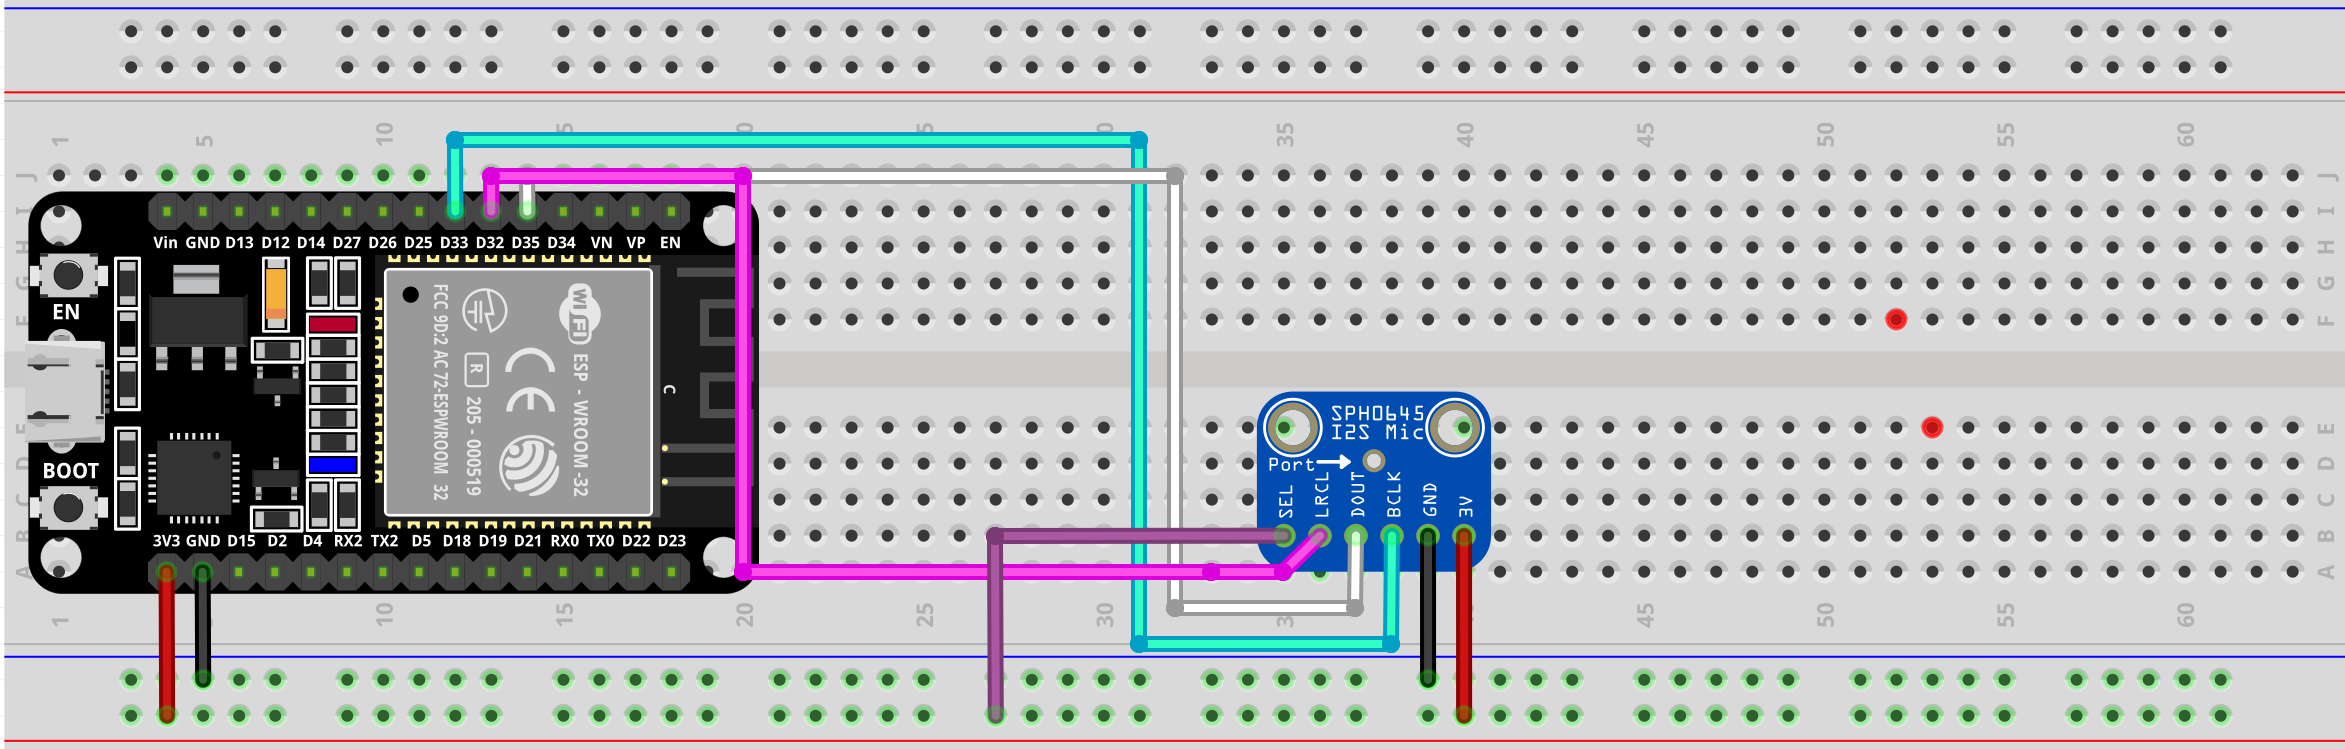
\includegraphics[width=\textwidth]{board_microfono.png}
    \caption{Collegamento fisico tra ESP32 e microfono I$^2$S (Adafruit SPH0645LM4H) su breadboard.}
    \label{fig:board_microfono}
  \end{figure} 

  \paragraph{Pinout del modulo microfonico.}
  Sulla scheda Adafruit, da sinistra a destra (come serigrafato) sono presenti i pin: SEL, LRCL (o LRCLK/WS), DOUT (o SD), BCLK (o SCK), GND, 3V.  
  DOUT è un’uscita a logica \SI{3.3}{\volt}; LRCLK e BCLK sono ingressi di clock; SEL è un ingresso statico per selezionare su quale slot (sinistro o destro) il microfono presenta i campioni sul bus I$^2$S.
  
  \paragraph{Mappatura dei segnali sull'ESP32.}
  La Tab.~\ref{tab:i2s_pins} riassume la corrispondenza dei pin usati, come nella figura. Le scelte rispettano i vincoli dell'ESP32 (evitando pin con funzioni di strapping all'avvio come GPIO15-12 o limitazioni di sola-lettura).
  
  \definecolor{lightgray}{RGB}{235,235,235}
  \definecolor{white}{RGB}{255,255,255}
  
  \begin{table}[H]
    \centering
    \label{tab:i2s_pins}
    \resizebox{\textwidth}{!}{%
    \begin{tabular}{|l|>{\columncolor{lightgray}}l|l|>{\columncolor{lightgray}}l|}
      \hline
    
      \textbf{Pin modulo} & \textbf{Segnale} & \textbf{Pin ESP32 (sigla serigrafata)} \\
      \hline
    
      3V   & Alimentazione \SI{3.3}{\volt}       & 3V3 \\
      \hline
    
      GND  & Riferimento di massa                & GND \\
      \hline
    
      BCLK & Bit Clock I$^2$S                    & GPIO14 (D14) \\
      \hline
    
      LRCL & Word-Select / LRCLK                 & GPIO25 (D25) \\
      \hline
    
      DOUT & Serial Data (uscita microfono)      & GPIO32 (D32) \\
      \hline
    
      SEL  & Selezione canale                    & GND $\rightarrow$ canale sinistro\\
      \hline
    
    \end{tabular}
    
    }
    \caption{Mappatura hardware dei pin I$^2$S tra ESP32 e microfono SPH0645LM4H.}
  
  \end{table}
  
  \noindent
  Il segnale SEL determina in quale slot vengono emessi i campioni audio: se portato a massa (SEL = GND) i dati escono sul canale sinistro,
  mentre a livello alto (SEL = 3V3) sul destro. \\
  Nel nostro schema è stato fissato a 3V3, quindi l’uscita è forzata a destra.
  Questo a seguito di alcuni test dove si è verificato che per qualche difformita nel IC il canale destro garantiva maggiore precisione.\\
  
  \paragraph{Dettagli elettrici e motivazioni delle scelte.}
  Il microfono Adafruit SPH0645LM4H funziona solo a 3.3 V: non sono previsti level shifter e un’alimentazione a 5 V lo danneggerebbe \cite{digikey-sheet}. L’assorbimento è dell’ordine dei mA, quindi l’uscita 3V3 dell’ESP32 è più che sufficiente \cite{digikey-sheet}.
    
  Per l’ESP32 si è scelto \textbf{GPIO14 come BCLK, GPIO25 come LRCLK e GPIO32} per il dato in ingresso.
    
  Infine, il microfono trasmette campioni a 24 bit allineati su frame da 32 come discusso precedentemente nella sezione \ref{subsec:mic}.
  
 
\subsection{Collegamento dell’amplificatore digitale I$^2$S}
\label{subsec:conn_amp}

La \autoref{fig:board_amp} mostra lo schema di cablaggio realizzato in \textbf{Fritzing} tra la breakout Adafruit basata sul chip \textbf{MAX98357A}
 (amplificatore in classe D con interfaccia I$^2$S) e la \textbf{ESP32}.  
L’interfaccia prevede tre linee digitali di segnale
(BCLK, LRCLK, DIN) e due linee di alimentazione (3V3, GND). Il modulo espone inoltre i pin di configurazione \textbf{GAIN} e \textbf{SD} (shutdown), 
che in questo caso non vengono utilizzati e restano flottanti.

\begin{figure}[H]
  \centering
  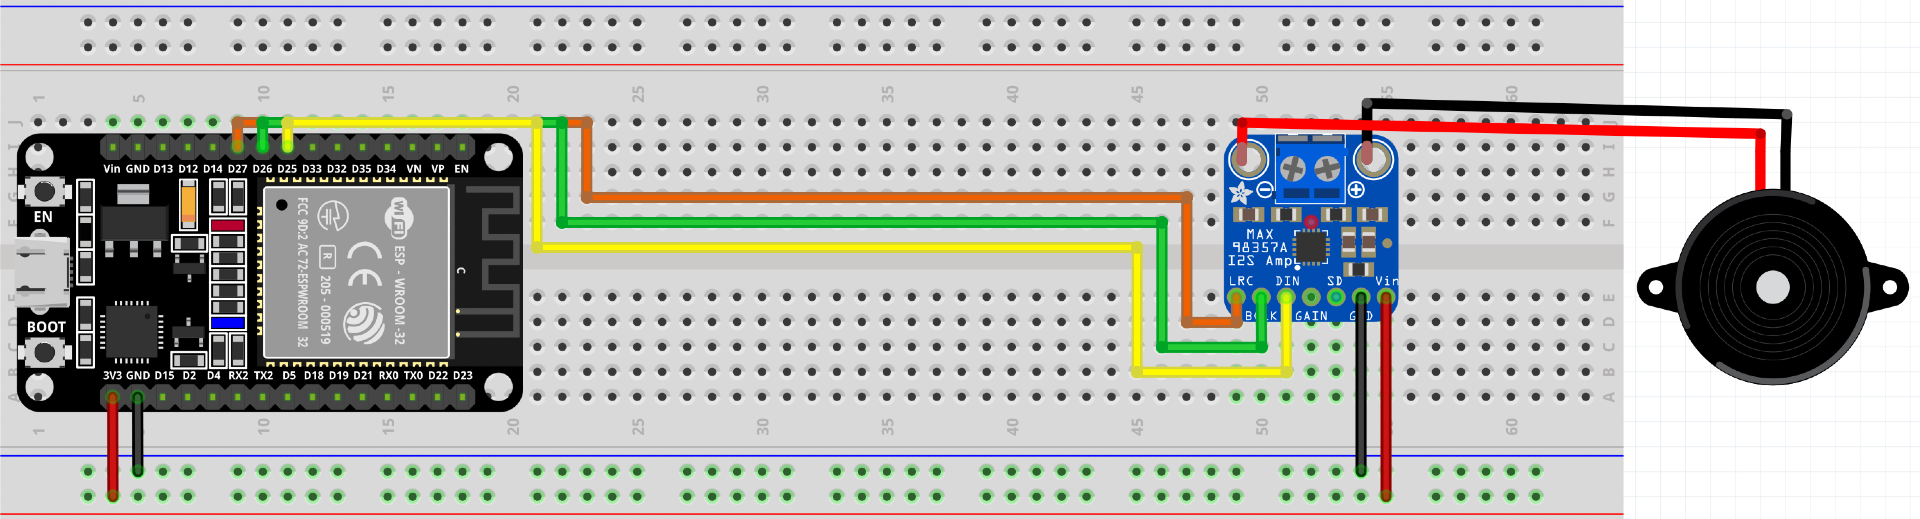
\includegraphics[width=\textwidth]{board_amp.png}
  \caption{Collegamento fisico tra ESP32 e amplificatore I$^2$S (Adafruit MAX98357A) su breadboard.}
  \label{fig:board_amp}
\end{figure} 

\paragraph{Pinout del modulo amplificatore.}
Sulla scheda Adafruit, da sinistra a destra (come serigrafato) sono presenti i pin: GAIN, SD, DIN, BCLK, LRCLK, GND, Vin.  
Il pin \textbf{DIN} è l’ingresso dati audio seriali (logica \SI{3.3}{\volt}); \textbf{BCLK} e \textbf{LRCLK} sono segnali di clock forniti dall’ESP32; \textbf{Vin} riceve l’alimentazione (3–5 V, compatibile col regolatore onboard).  
I pin GAIN e SD sono opzionali: GAIN permette di configurare il guadagno interno tramite resistenze, mentre SD forza il chip in modalità risparmio energetico.

\paragraph{Mappatura dei segnali sull'ESP32.}
La Tab.~\ref{tab:i2s_pins_amp} riassume la corrispondenza dei pin usati, come nello schema. Anche in questo caso la scelta dei GPIO tiene conto delle raccomandazioni di Espressif, evitando pin con funzioni critiche all’avvio.


\begin{table}[H]
  \centering
  \label{tab:i2s_pins_amp}
  \resizebox{\textwidth}{!}{%
  \begin{tabular}{|l|>{\columncolor{lightgray}}l|l|}
    \hline
  
    \textbf{Pin modulo} & \textbf{Segnale} & \textbf{Pin ESP32 (sigla serigrafata)} \\
    \hline
  
    Vin  & Alimentazione \SI{3.3}{\volt} / \SI{5}{\volt} & 3V3 \\
    \hline
  
    GND  & Riferimento di massa                        & GND \\
    \hline
  
    BCLK & Bit Clock I$^2$S                            & GPIO14 (D14) \\
    \hline
  
    LRCLK & Word-Select / LRCLK                        & GPIO25 (D25) \\
    \hline
  
    DIN  & Serial Data (ingresso audio)                & GPIO26 (D26) \\
    \hline
  
    SD   & Shutdown (non connesso)                     & -- \\
    \hline
  
    GAIN & Configurazione guadagno (non connesso)      & -- \\
    \hline
  
  \end{tabular}
  }
  \caption{Mappatura hardware dei pin I$^2$S tra ESP32 e amplificatore MAX98357A.}
\end{table}

\noindent
Il collegamento all’altoparlante avviene direttamente dai terminali di uscita del modulo (OUT$+$, OUT$-$), come mostrato in figura.  
Essendo un amplificatore in classe D capace di pilotare piccoli altoparlanti (4–8~$\Omega$, fino a circa \SI{3}{W} a 5 V),
 non è necessaria ulteriore elettronica per il collegamento all'altoparlante.

\paragraph{Dettagli elettrici e motivazioni delle scelte.}
Il MAX98357A accetta alimentazione sia a 3.3 V che a 5 V \cite{maxim-datasheet}: in questo schema si è scelto di usare il \textbf{3V3 dell’ESP32} per semplicità,
 tenendo conto che ciò limita la potenza massima erogabile all’altoparlante e considerando che in
  una reale applicazione a scopo industriale si utilizzerebbero amplificatori da \~ 230 V.  
Il consumo è nell’ordine di poche decine di mA a volume medio, quindi l’uscita 3V3 dell’ESP32 è sufficiente in prototipazione.  



\subsection{Sistema di segnalazione LED}
\label{subsec:led_system}

La \autoref{fig:board_led} mostra lo schema di cablaggio realizzato in \textbf{Fritzing} tra la scheda \textbf{ESP32} e tre LED collegati su breadboard.  
Il sistema fornisce un feedback visivo sullo stato di decodifica del segnale audio, a supporto del protocollo discusso nella sezione \ref{sec:filtraggio}.  

\begin{figure}[H]
  \centering
  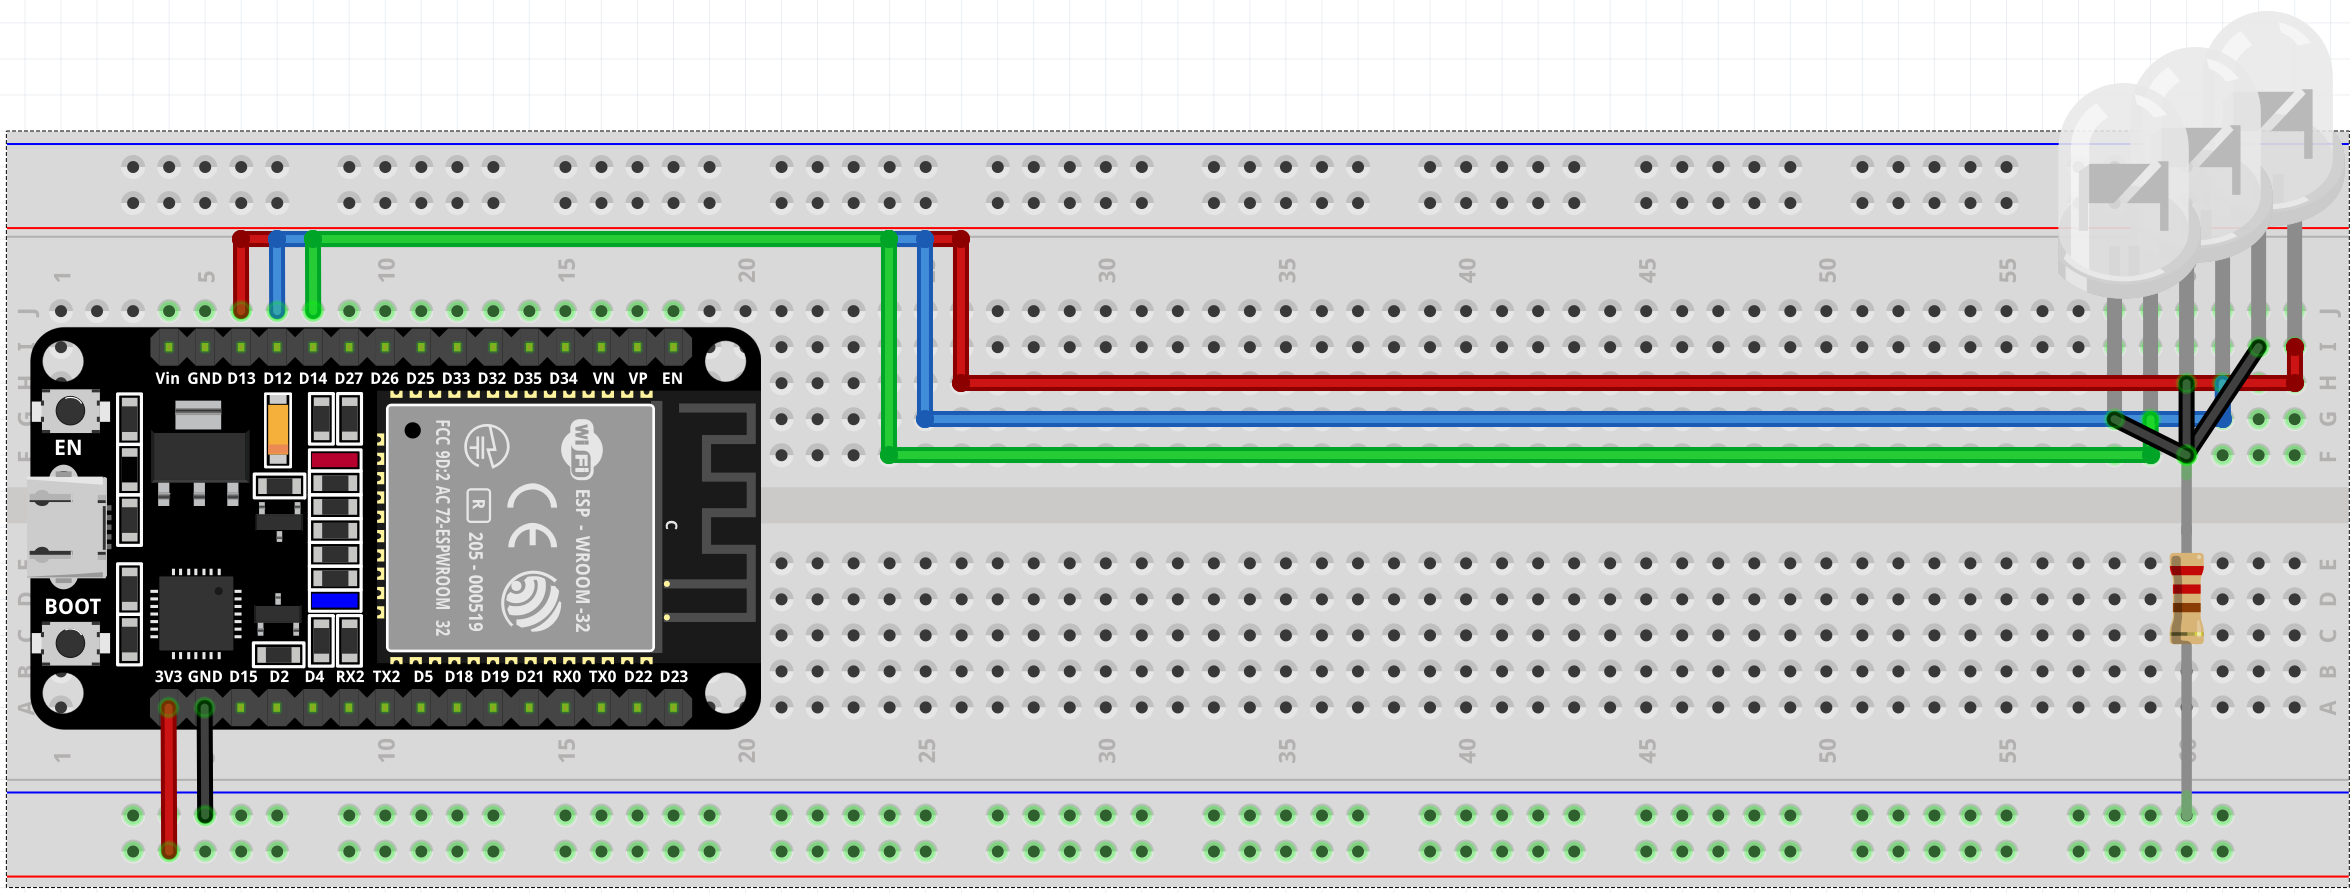
\includegraphics[width=\textwidth]{board_led.png}
  \caption{Collegamento fisico tra ESP32 e LED di segnalazione su breadboard.}
  \label{fig:board_led}
\end{figure} 

\paragraph{Funzionamento del sistema.}
Sono stati utilizzati tre LED di colore diverso (verde, blu e rosso) per rappresentare in modo immediato lo stato di elaborazione:  
\begin{itemize}
  \item LED verde: il segnale è stato decodificato correttamente;
  \item LED blu: il segnale è in fase di decodifica;
  \item LED rosso: il segnale non ha superato il controllo dell’interpolazione parabolica e non è stato decodificato correttamente.
\end{itemize}

\paragraph{Mappatura dei segnali sull'ESP32.}
La Tab.~\ref{tab:led_pins} riassume la corrispondenza dei pin usati per il pilotaggio dei tre LED, come nello schema in figura.  
Ogni LED è collegato in serie a una resistenza di limitazione, necessaria a ridurre la corrente entro i limiti di sicurezza per i GPIO dell’ESP32 (massimo \SI{12}{mA} consigliati).

\definecolor{lightgray}{RGB}{235,235,235}
\definecolor{white}{RGB}{255,255,255}

\begin{table}[H]
  \centering
  \label{tab:led_pins}
  \resizebox{\textwidth}{!}{%
  \begin{tabular}{|l|>{\columncolor{lightgray}}l|l|}
    \hline
  
    \textbf{LED} & \textbf{Funzione} & \textbf{Pin ESP32 (sigla serigrafata)} \\
    \hline
  
    Verde & Decodifica corretta & GPIO14 (D14) \\
    \hline
  
    Blu   & Decodifica in corso & GPIO27 (D27) \\
    \hline
  
    Rosso & Errore di decodifica & GPIO26 (D26) \\
    \hline
  
  \end{tabular}
  }
  \caption{Mappatura hardware dei pin di uscita dell’ESP32 verso i LED di stato.}
\end{table}

\paragraph{Dettagli elettrici e motivazioni delle scelte.}
Ciascun LED è collegato al rispettivo GPIO tramite una resistenza da \SI{220}{\ohm}, sufficiente a limitare la corrente senza ridurre eccessivamente la luminosità.  
I pin \textbf{GPIO14, GPIO27 e GPIO26} sono stati scelti in quanto liberi da vincoli di boot e comunemente usati per uscite digitali.  

\subsection{Bottone di Hotspot}
\label{subsec:button_hotspot}

La \autoref{fig:board_bottone} mostra il collegamento su breadboard di un pulsante e due LED all’ESP32.  
Il pulsante è collegato al pin \textbf{GPIO34 (D34)} e consente di abilitare la modalità \textit{hotspot} prevista dal protocollo (\ref{sec:livello_link}).  

\begin{figure}[H]
  \centering
  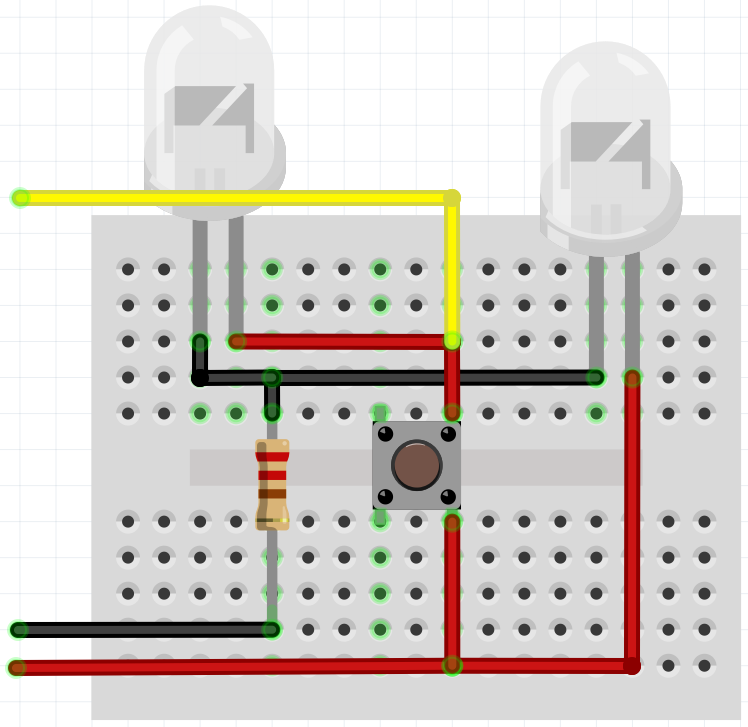
\includegraphics[width=0.35\textwidth]{board_bottone.png}
  \caption{Schema di collegamento del bottone e dei LED di stato per la modalità hotspot.}
  \label{fig:board_bottone}
\end{figure}

Il LED giallo, a sinistra, indica l’attivazione dell’hotspot e si accende solo alla pressione del pulsante.  
Il LED a destra segnala invece lo stato di alimentazione della scheda, acceso quando l’ESP32 è in funzione e spento in assenza di alimentazione.  
 
\subsection{Circuito completo}
\label{subsec:circuito_completo}

La \autoref{fig:board_completa} riassume l’intero sistema realizzato su breadboard, integrando in un 
unico schema tutte le funzionalità descritte nelle sezioni precedenti. L’\textbf{ESP32}, alimentato da 
un pacco batterie AAA, costituisce il cuore del circuito e gestisce sia la parte di acquisizione sia quella 
di elaborazione e segnalazione. \\
Il microfono \textbf{I²S} raccoglie il segnale audio e lo invia al microcontrollore, 
che a sua volta lo riproduce attraverso l’amplificatore digitale \textbf{MAX98357A} collegato a un piccolo altoparlante.\\
 In parallelo, il sistema integra un’interfaccia visiva con tre LED che indicano lo stato della decodifica, insieme a un
  pulsante dedicato all’attivazione della modalità \textit{hotspot}, il cui stato è reso evidente da un ulteriore LED giallo. \\
  Tutti i collegamenti sono realizzati su breadboard, con le linee di alimentazione distribuite ai vari moduli e i segnali instradati 
  verso i pin dell’ESP32, tra cui il \textbf{GPIO34}, correttamente utilizzato come ingresso per il pulsante. In questo modo il circuito 
  offre un esempio completo di integrazione tra acquisizione, elaborazione, riproduzione e interfaccia utente, consentendo il passaggio 
  fluido dall’ascolto alla decodifica, fino alla segnalazione visiva e al controllo della connessione wireless.

\begin{figure}[H]
  \centering
  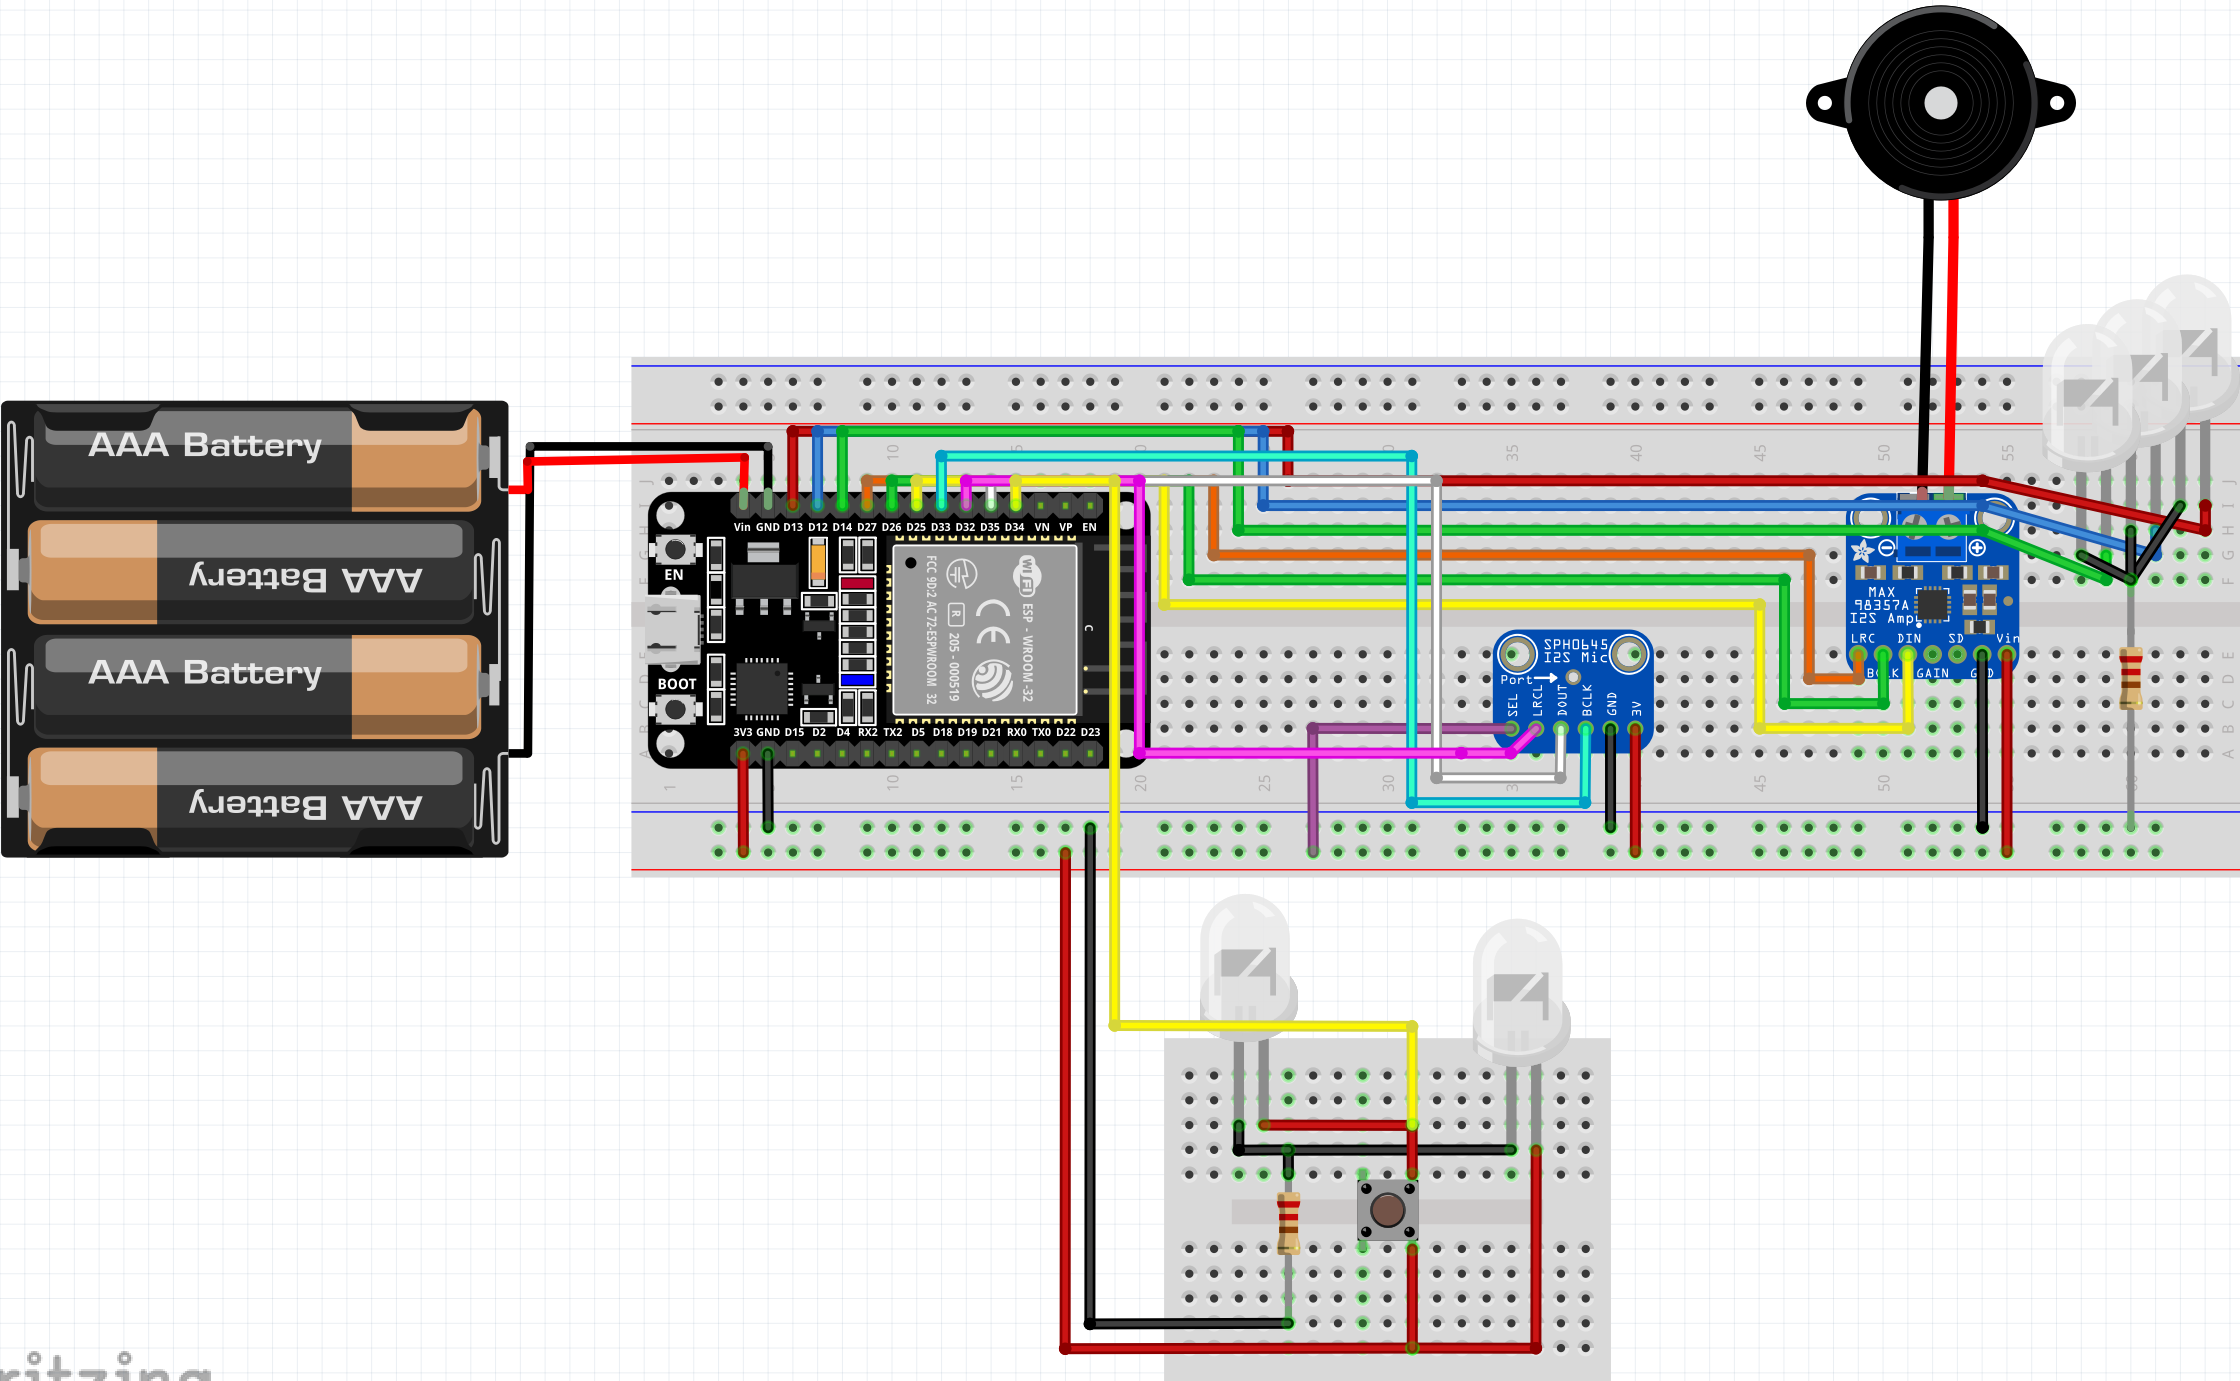
\includegraphics[width=\textwidth]{board_completa.png}
  \caption{Schema del circuito completo con ESP32, microfono I²S, amplificatore MAX98357A, LED di stato e pulsante di hotspot.}
  \label{fig:board_completa}
\end{figure}

\subsection{Realizzazione del PCB}
\label{subsec:pcb_completo}

Dopo aver completato lo schema su breadboard, il progetto è stato trasferito in \textbf{vista PCB} 
all’interno di Fritzing, con le dovute modifiche, ottenendo così una scheda stampata ordinata e compatta, come mostrato in \autoref{fig:pcb_completo}.\\ 
In questa configurazione l’\textbf{ESP32} rimane al centro della scheda, con le piste di segnale distribuite verso i moduli periferici: 
i LED di stato con le relative resistenze sono disposti lungo il bordo destro per facilitare la visibilità [LED-1-2-3], mentre il pulsante di hotspot 
è collocato nella parte inferiore [S2] insieme al LED [LED4] che ne segnala l’attivazione. \\
Il layout delle piste è stato ottimizzato per ridurre le interferenze e mantenere separati i percorsi di potenza da quelli di segnale.\\
Questo passaggio è stato fatto per poter permettere una futura produzione in serie del dispositivo.

\begin{figure}[H]
  \centering
  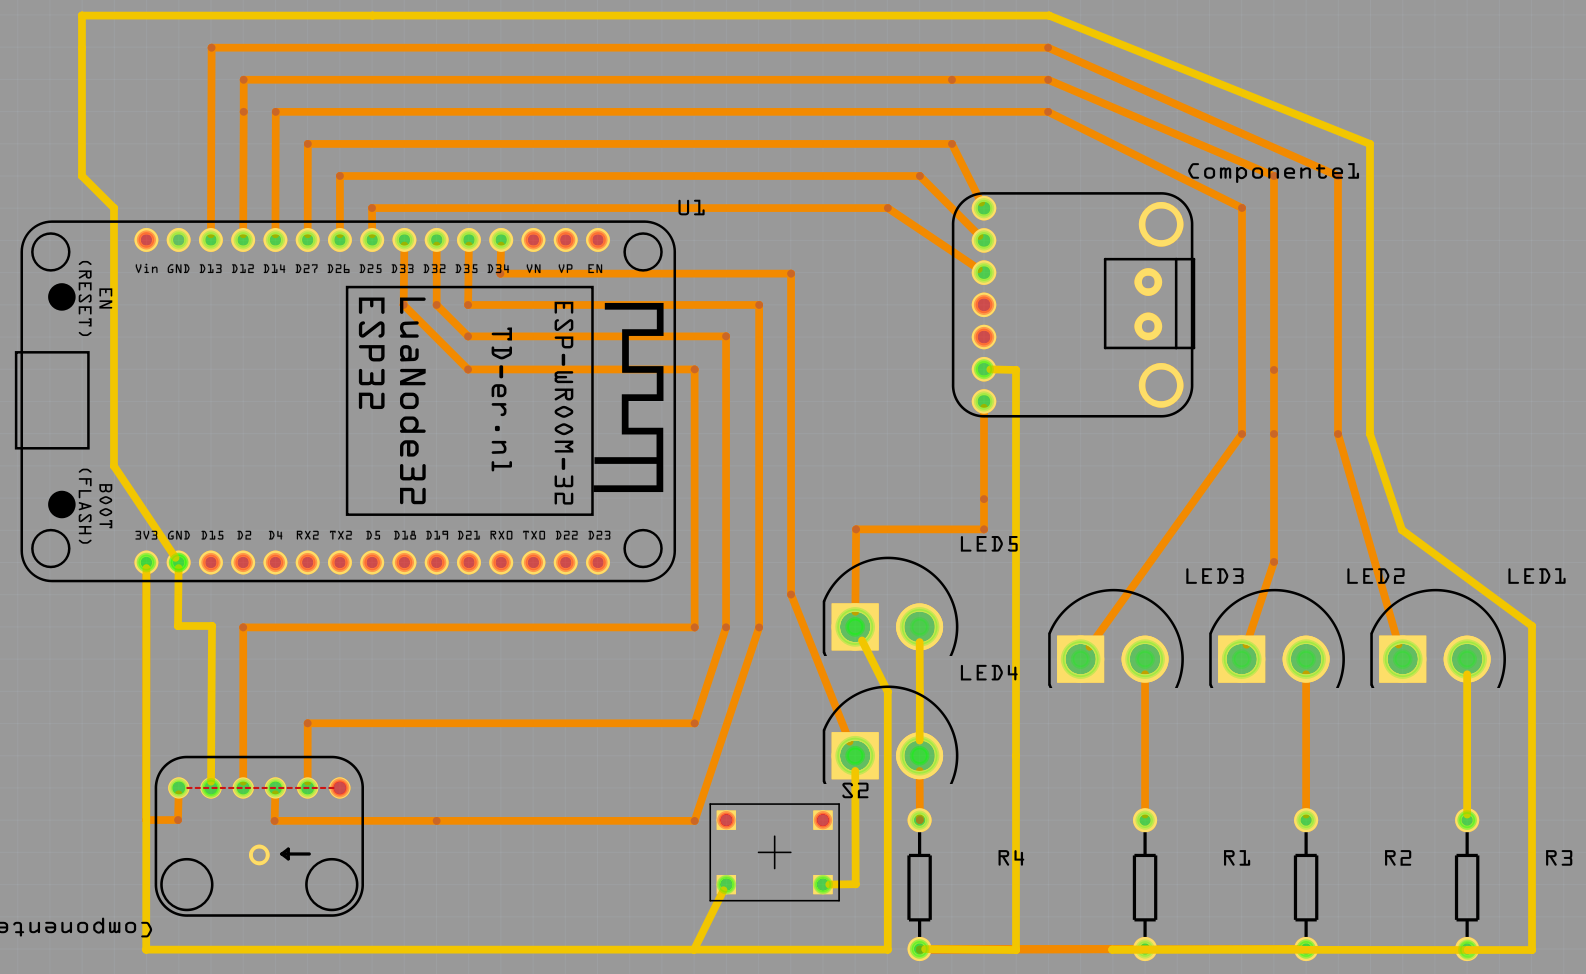
\includegraphics[width=\textwidth]{pcb_completo.png}
  \caption{Layout del circuito stampato (PCB), con ESP32, LED di stato, pulsante di hotspot e connettori di alimentazione.}
  \label{fig:pcb_completo}
\end{figure}

\chapter{Implementazione Software: Design del Protocollo}
\label{chap:implementazione_software}

\section{Architettura generale del sistema}

Il software è stato sviluppato in linguaggio \textbf{C}, scelta che ha permesso di avere un controllo diretto sull’hardware dell’ESP32,
ottenendo esecuzioni prevedibili ed un uso minuzioso delle risorse. \\
L’utilizzo del C ha inoltre garantito maggiore leggerezza rispetto al C++ e una buona portabilità, grazie alla disponibilità di librerie 
già consolidate in ambito firmware.  

Alcune librerie Arduino originariamente scritte in C++ sono state adattate in C, questo per permettere la compilazione del codice.\\
Allo stesso tempo, l’uso del framework Arduino su 
ESP32 ha offerto vantaggi importanti tra cui: documentazione estesa, supporto diretto alle periferiche del microcontrollore e una 
community ampia, che ha velocizzato la fase di sviluppo. \\

Per lo sviluppo è stato utilizzato \textit{Visual Studio Code}, scelto per l’ampia disponibilità di estensioni.
In particolare, l’integrazione con \textbf{PlatformIO} ha reso più semplice la gestione del progetto: compilazione, caricamento e debugging sono stati 
unificati in un unico ambiente; la gestione automatica delle librerie e delle dipendenze ha permesso uno sviluppo più rapido ed organizzato.\\ 

L’architettura complessiva si basa su moduli separati e specializzati, ognuno responsabile di una parte precisa del protocollo. 
Questo approccio modulare ha garantito una migliore manutenibilità del codice e ha semplificato l’integrazione tra i diversi livelli funzionali 
descritti in \autoref{chap:design_protocollo}, il cui codice sorgente completo è riportato in \autoref{appendice:repository}.\\


\section{Emissione dei toni}

L’uscita audio discussa nella \autoref{sec:uscita_livello_fisico} è gestita dal modulo \textbf{audio\_driver}, 
responsabile dell’inizializzazione del bus I\textsuperscript{2}S e della generazione in tempo reale delle sinusoidi che rappresentano i bit. \\
La funzione \textbf{play\_two\_tones} produce due toni simultanei, richiedendo come parametri le due frequenze delle quali dovrà generare le sinusoidi.
La generazione del segnale avviene con persistenza di fase, evitando discontinuità tra un’emissione e la successiva. 


\begin{minted}[linenos,breaklines]{c}
void play_two_tones(int freq1, int freq2) {
    if(freq1 == 0 && freq2 == 0){
        delay(80);
    } else {
        const float tone_duration = 0.024f;
        const int tone_samples = (int)(G_SAMPLE_RATE * tone_duration);
        const int tone_buffer_size = tone_samples * 2;
        int16_t tone_buffer[tone_buffer_size];
    \end{minted}
Le variabili sotto garantiscono la continuità di fase tra chiamate successive della funzione:
\begin{minted}[linenos,breaklines]{c}
        static float phase1 = 0.0f;
        static float phase2 = 0.0f;
        const float inc1 = 2.0f * PI * freq1 / G_SAMPLE_RATE;
        const float inc2 = 2.0f * PI * freq2 / G_SAMPLE_RATE;
    \end{minted}
Questo frammento di codice mostra la generazione del buffer di campioni,
 che viene poi scritto sul bus I\textsuperscript{2}S:
\begin{minted}[linenos,breaklines]{c}
        for (int i = 0; i < tone_samples; i++) {
            float mixed = sinf(phase1) + sinf(phase2);
            int16_t sample = (int16_t)(3000 * (mixed / 2.0f));
            tone_buffer[2 * i] = sample;
            tone_buffer[2 * i + 1] = sample;
            phase1 += inc1;
            if (phase1 >= 2.0f * PI) phase1 -= 2.0f * PI;
            phase2 += inc2;
            if (phase2 >= 2.0f * PI) phase2 -= 2.0f * PI;
        }
        size_t bytes_written = 0;
        i2s_write(I2S_NUM, tone_buffer, sizeof(tone_buffer), &bytes_written, portMAX_DELAY);
    }
}
\end{minted}

L’ampiezza massima del segnale è limitata a un valore inferiore a 32767 per evitare saturazioni sul DAC, questa conclusione deriva
 da test che hanno mostrato come 
 il fattore di scaling a \textbf{3000} garantisce \textbf{headroom sufficiente}. Quando entrambe le frequenze sono nulle,
  la routine introduce una pausa di \textbf{80 ms}, che equivale a una “inattività” progettata per separare gruppi di
   simboli o pacchetti.

\section{Campionamento e bufferizzazione}

Il percorso inverso, ovvero l’acquisizione dei toni ricevuti, discusso nella \autoref{sec:ingresso_livello_fisico} come l'ingresso del Livello Fisico 
è affidato al \textbf{reader}.  \\ 
Il modulo crea due buffer circolari tra cui effettua un meccanismo di \textbf{swapping sincronizzato}: mentre uno viene riempito dal task di I\textsuperscript{2}S, 
l’altro è disponibile per l’elaborazione FFT, questo avviene attraverso un insieme di variabili rese \textbf{extern} e mediante l'uso di un \textbf{puntatore} 
con attributo \textbf{extern} che punta sempre al buffer pronto, cosi da renderlo disponibile alla funzione richiedente senza che questa entri nella 
logica del reader. \\

\begin{minted}[linenos,breaklines]{c}
extern volatile int data_ready;
extern volatile int status_flag;
extern complex_g3_t *array_ready;
\end{minted}

La funzione \textbf{reader\_task} legge i campioni dal bus I\textsuperscript{2}S, li converte in numeri complessi e li memorizza nel buffer corrente.\\

\begin{minted}[linenos,breaklines]{c}
static void reader_task(void *param) {
    size_t bytes_read;
    int32_t dma_buffer[DMA_BUFFER_SIZE / 4];
    static float dc_mean = 0.0f;
    const float alpha = 1.0f / 1024.0f;
    while (1) {
        i2s_read(I2S_PORT, (void*)dma_buffer, DMA_BUFFER_SIZE, &bytes_read, portMAX_DELAY);
        int samples = bytes_read / 4;
        for (int i = 0; i < samples; i++) {
            int32_t s32 = dma_buffer[i] >> 8;
            float x = (float)(s32 >> 12);
            dc_mean += alpha * (x - dc_mean);
            float val = x - dc_mean;
            current_data[counter].re = (double)val;
            current_data[counter].im = 0.0;
            counter++;
            if (counter >= ARRAY_ELEMENTS) {
                data_ready = 1;
                swap_array();
                counter = 0;
            }
        }
    }
}
\end{minted}

L’eliminazione della componente DC avviene con una media mobile parametrizzata da \textbf{alpha}, \\ 
il quale viene; i campioni centrati vengono convertiti in numeri complessi con parte immaginaria nulla per l’elaborazione spettrale.\\
L’uso di \textbf{swap\_array} consente di non perdere alcun campione e di garantire un’elaborazione a flusso continuo.  \\

\begin{minted}[linenos,breaklines]{c}
 static void swap_array(void) {
     array_ready = current_data;
     current_data = (current_data == main_array) ? secondary_array : main_array;
 }
 \end{minted}

\begin{figure}[H]
    \centering
    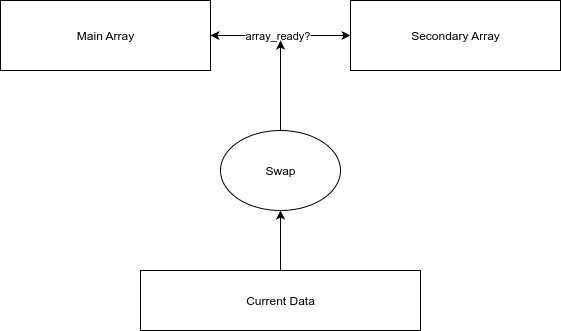
\includegraphics[width=0.6\textwidth]{immagini/swapping_array.png}
    \caption{Swapping degli array di campioni}
    \label{fig:swapping_array}
\end{figure}

\section{Trasformata veloce di Fourier}
Altro aspetto critico del Livello Fisico è la trasformata rapida di Fourier (FFT), che converte i campioni temporali in rappresentazioni spettrali. 
Cosi come discusso nella \autoref{par: fft_calcolo}, l’implementazione adottata è una versione personalizzata dell’algoritmo di Cooley–Tukey, ottimizzata per
 il contesto real-time e per la risoluzione richiesta. \\
 L'analisi frequenziale viene eseguita nel modulo \textbf{fft.c}, questa include due funzioni principali \textbf{FFT\_get\_twiddle\_factors} e \textbf{FFT\_calculate}. \\

\begin{minted}[linenos,breaklines]{c}
void FFT_calculate (complex_g3_t *x, long N, complex_g3_t *X,
                    complex_g3_t *scratch, complex_g3_t *twiddles){
    int k, m, n;
    int skip;
    boolean evenIteration = N & 0x55555555;
    complex_g3_t* E;
    complex_g3_t* Xp, *Xp2, *Xstart;
    if (N == 1){
        X[0] = x[0];
        return;
    }
    E = x;
    for (n = 1; n < N; n = n * 2){
        Xstart = evenIteration ? scratch : X;
        skip = N / (2 * n);
        Xp = Xstart;
        Xp2 = Xstart + N / 2;
        for (k = 0; k < n; k++){
            double tim = twiddles[k * skip].im;
            double tre = twiddles[k * skip].re;
            for (m = 0; m < skip; ++m){
                complex_g3_t* D = E + skip;
                double dre = D->re * tre - D->im * tim;
                double dim = D->re * tim + D->im * tre;
                Xp->re  = E->re + dre;
                Xp->im  = E->im + dim;
                Xp2->re = E->re - dre;
                Xp2->im = E->im - dim;
                ++Xp; ++Xp2; ++E;
            }
            E += skip;
        }
        E = Xstart;
        evenIteration = !evenIteration;
    }
}
\end{minted}

Lo schema fa uso di array globali per l’uscita e per lo spazio temporaneo, così da evitare allocazioni
 dinamiche che in un contesto real-time sarebbero troppo costose.\\
  Il flag \textbf{evenIteration} serve 
 a gestire il ping-pong tra l’array risultato e quello di appoggio:
 in questo modo si alternano i ruoli dei due buffer a ogni passo, senza dover copiare dati inutilmente.


 \section{Decodifica spettrale}

 Le frequenze individuate dalla trasformata passano al modulo \textbf{decoder}, 
 che ha il compito di capire se un picco spettrale corrisponde davvero a un tono
  del protocollo oppure se si tratta di rumore. Questa logica è implementata nella funzione
   \textbf{check\_active\_frequencies}, che lavora in tre fasi: calcolo della soglia dinamica,
    controllo dei massimi locali e interpolazione del picco confermato.  
 
 \begin{minted}[linenos,breaklines]{c}
 struct_interpolated_frequency check_active_frequencies(
         complex_g3_t *data, int bin_1, int bin_2,
         int id, double noise_floor){
     int i, j;
     struct_interpolated_frequency detected_freq;
     detected_freq.work = 0;
     detected_freq.frequency = -1.0;
     detected_freq.estimated_amplitude = -1.0;
     detected_freq.dynamic_amplitude_threshold = -1.0;
 \end{minted}
 
 La funzione crea una struttura \textbf{detected\_freq} che conterrà il risultato. 
 Tutti i campi sono inizializzati a valori “non validi” (ad esempio -1.0) così che, 
 se nessuna frequenza viene trovata, il chiamante può accorgersene immediatamente.  
 
 \begin{minted}[linenos,firstnumber=14,breaklines]{c}
     for (j = bin_1; j <= bin_2; j++){
         double freq = (double)(FS * j) / NN;
         double amp = complex_magnitude(data[j]);
 \end{minted}
 
 Il ciclo scorre i bin tra \textbf{bin\_1} e \textbf{bin\_2} che, come discusso nel \autoref{subsec:filtraggio} i bin sono 
 la rappresentazione discreta della frequenza nello spettro ottenuto dalla FFT.
 \begin{equation}
    bin[i] = (FS * i) / NN = (48000 * i) / 512 = 93.75 * i.
 \end{equation}
  La formula calcola la frequenza corrispondente a ogni bin, dove \textbf{FS} è la frequenza di campionamento e \textbf{NN} il numero di punti della FFT.\\
  Il BIN è quindi un indice che rappresenta una specifica frequenza nell'array risultante dalla FFT.\\
   La funzione \textbf{complex\_magnitude} calcola il modulo del numero complesso associato al bin corrente, che rappresenta l’ampiezza del segnale a quella frequenza.\\

 \begin{minted}[linenos,firstnumber=18,breaklines]{c}
         if(G_LINEAR_REGRESSION_MODE == 0){
             double dynamic_amplitude_threshold = noise_floor * 8.0;
             if (amp > dynamic_amplitude_threshold){
                 for(i = j-6; i < j + 6 && complex_magnitude(data[i]) <= amp; i++) {}
                 if (i == j+6){
                     detected_freq = interpolate_peak_frequency(data, j, FS, NN);
                     detected_freq.dynamic_amplitude_threshold = dynamic_amplitude_threshold;
                     detected_freq.work = 1;
                     return detected_freq;
                 }
             }
 \end{minted}
 
La soglia dinamica (dynamic\_amplitude\_threshold) è otto volte il \textbf{noise\_floor}.
 Una volta superata la soglia, viene controllata una finestra di 12 bin, come rappresentato in \autoref{fig:bins_local_peak} (sei a sinistra e sei a destra) 
 per assicurarsi che il valore corrente sia davvero un massimo locale. \\
Solo in questo caso si invoca \textbf{interpolate\_peak\_frequency}, le quali motivazioni e funzionamento sono spiegate nel \autoref{par: interpolazione_parabolica},
 che con una formula di interpolazione parabolica calcola la frequenza “vera”, 
per sopperire alla bassa risoluzione spettrale, questa tecnica, quindi fornisce una precisione sub-bin, cioè di una frequenza intermedia tra due bin adiacenti.\\  

 
 Infine, se nessuna frequenza valida è trovata, la funzione ritorna la struttura con i valori -1.0.  
 
 \section{Traduzione frequenza-bit}
 
 Una volta isolati i picchi, i moduli riguardanti il Livello Fisico lasciano spazio ai \textbf{moduli del Livello Bit} il primo passo è tradurli in 
 \textbf{Signal Codes} come nella seguente tabella.
  Questa operazione è svolta dal modulo \textbf{bit\_freq\_codec}, e in particolare dalla funzione \textbf{interpret\_bits}.  

  \definecolor{lightgray}{RGB}{235,235,235}
\definecolor{white}{RGB}{255,255,255}


  \begin{table}[H]
    \centering
    \label{tab:freq_codici_divisi}
    \begin{tabular}{|l|>{\columncolor{lightgray}}l|>{\columncolor{lightgray}}l|}
    \hline
    \textbf{Frequenza} & \textbf{Signal Code (0)} & \textbf{Signal Code (1)} \\
    \hline
    1400 & (0) & \\
    1800 & (1) & \\
    2200 & (2) & \\
    2600 & (3) & \\
    3000 & (4) & \\
    3400 & (5) & \\
    3800 & (6) & \\
    4200 & (7) & \\
    4600 & (8) & \\
    5000 & & (9) \\
    5400 & & (10) \\
    5800 & & (11) \\
    6200 & & (12) \\
    6600 & & (13) \\
    7000 & & (14) \\
    7400 & & (15) \\
    7800 & & (16) \\
    8200 & & (17) \\
    \hline
    \end{tabular}
    \caption{Mappatura frequenze con divisione dei Signal Code in 0 e 1}
\end{table}



 \begin{minted}[linenos,breaklines]{c}
 int interpret_bits(int freqs[3]){
     int count = 0;
     int active[3] = {0};
     for (int i = 0; i < 3; ++i) {
         if (freqs[i] > 0) {
             active[i] = 1;
             count++;
         }
     }
 \end{minted}
 
 La funzione riceve in ingresso un array di tre frequenze, dove la prima posizione è riservata alla \textbf{frequenza dello zero},
 la seconda alla \textbf{frequenza della portante} questa serve ad identificare il canale tra (master, slave ed config) più che alla creazione del Signal Code,
    e la terza alla \textbf{frequenza dell'uno}. 
    Il contatore \textbf{count} tiene traccia del numero di toni attivi: se è diverso da due, oppure i toni ricevuti sono quelli esterni,
    quindi senza tono che indica il canale, allora il simbolo non è valido.
 
 \begin{minted}[linenos,firstnumber=10,breaklines]{c}
     if (count == 2) {
         if (active[0] && active[1] && !active[2]){
             if(freqs[0] < MASTER_BASE + (TONE_STEP*19) && freqs[1] == MASTER_BASE){
                 return (freqs[0]-MASTER_BASE)/(TONE_STEP);
             }
             if(freqs[0] < SLAVE_BASE + (TONE_STEP*19) && freqs[1] == SLAVE_CARRIER){
                 return (freqs[0]-SLAVE_BASE)/(TONE_STEP);
             }
             if(freqs[0] < CONFIG_BASE + (TONE_STEP*19) && freqs[1] == CONFIG_CARRIER){
                 return (freqs[0]-CONFIG_BASE)/(TONE_STEP);
             }
         }
 \end{minted}
 
 Se ci sono due frequenze attive, si controlla quale delle tre posizioni è spenta e si determina il ruolo: \textbf{master}, \textbf{slave} o \textbf{config}. \\
 Il calcolo restituisce un il \textbf{Signal Code} che rappresenta \textbf{quanti zeri o uno consecutivi} sono codificati in quel simbolo come è stato illustrato 
 nella \autoref{tab:freq_codici}.
 
 \begin{minted}[linenos,firstnumber=23,breaklines]{c}
         if (!active[0] && active[1] && active[2]){
             if(freqs[2] < MASTER_BASE + (TONE_STEP*19) && freqs[1] == MASTER_BASE){
                 return (freqs[2]-MASTER_BASE)/(TONE_STEP);
             }
             if(freqs[2] < SLAVE_BASE + (TONE_STEP*19) && freqs[1] == SLAVE_CARRIER){
                 return (freqs[2]-SLAVE_BASE)/(TONE_STEP);
             }
             if(freqs[2] < CONFIG_BASE + (TONE_STEP*19) && freqs[1] == CONFIG_CARRIER){
                 return (freqs[2]-CONFIG_BASE)/(TONE_STEP);
             }
         }
         return -2;
     } else if (count == 3) {
         return -2;
     } else {
         return -3;
     }
 }
 \end{minted}
 
 I valori negativi gestiscono gli errori: \textbf{-2} significa che la combinazione di frequenze non è valida, mentre \textbf{-3} indica 
 che non ci sono abbastanza toni per interpretare un simbolo.\\  
 
 Infine, la conversione inversa è svolta da \textbf{frequency\_coder}, che genera le coppie di frequenze a partire da un
  \textbf{Signal Code} e dal ruolo del canale. 
 

\section{Ricevimento e trasmissione dei bit (Packers)}
\subsection{Ricezione dei bit}
Terminata la decodifica, i \textbf{Signal Code} vengono accumulati in buffer a sette bit dal modulo \textbf{bit\_input\_packer}. \\ 
Un aspetto sofisticato di questo componente è la gestione del flush: questo aspetta l'arrivo di un Signal Code 8 che rappresenta 21 zero consecutivi,
ma è condizionato da un timeout, utile quando i toni cessano di arrivare ma il Code 8 non è arrivato, a causa di qualche interferenza. \\
 L’algoritmo controlla costantemente l’istante dell’ultimo bit per ogni canale, e se per più di un secondo non sopraggiungono nuovi simboli effettua la conversione in ASCII.
Questa ne è l'implementazione:

\begin{minted}[linenos,breaklines]{c}
static bool timeout_flush_if_needed(BitPacker* packer,
                                     const char* label,
                                     bool* timeout_armed,
                                     uint64_t last_bit_ms,
                                     bool no_new_bit_this_tick){
    if (!*timeout_armed) return false;
    if (!no_new_bit_this_tick) return false;
    uint64_t tnow = now_ms();
    if ((tnow - last_bit_ms) < TIMEOUT_MS) return false;
    bool ok = flush_and_convert_to_ascii(packer, label);
    *timeout_armed = false;
    return ok;
}
\end{minted}

Quando il flush viene eseguito, la routine \textbf{flush\_and\_convert\_to\_ascii} 
trasferisce il contenuto della struttura in array di caratteri, inoltre ne verifica la qualità del pacchetto accertandosi che non ci siano caratteri non stampabili.\\
 La funzione ritorna \textbf{true} se il pacchetto è valido, \textbf{false} altrimenti.

\subsection{Trasmissione dei bit}

 L'inversa della fase di ricevimento dei bit, è la fase di trasmissione dei bit, ovvero l’impacchettamento dei bit in uscita in \textbf{Signal Code}, 
 è svolto dal modulo 
 \textbf{bit\_output\_packer}, che comprime i bit in \textbf{Signal Code} applicando una semplice forma di \textbf{run-length}
  encoding e replicando ogni codice più volte per incrementare la robustezza in presenza di rumore, cosi che venga trasmesso dal livello fisico 
  per 3 volte consecutivamente, come illustrato in figura \autoref{fig:finestra_ascolto} ogni codice verrà trasmesso per un tempo di 24ms, quindi ritrasmettendo 
  per 3 volte ogni codice, si avrà una finestra di ascolto di 72ms per ogni codice.\\

  \begin{figure}[H]
    \centering
    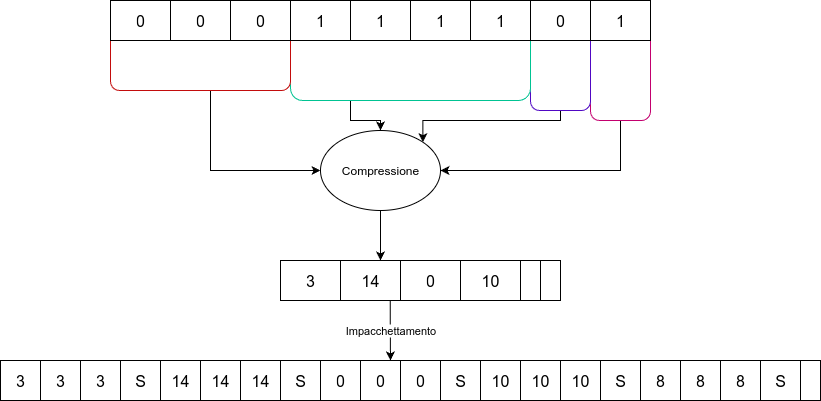
\includegraphics[width=0.75\textwidth]{immagini/run_length.png}
    \caption{Compressione ed impacchettamento mediante Algoritmo Run-Length S= Silenzio}
    \label{fig:run_length}
\end{figure}

   Nel seguente frammento  è mostrata la parte conclusiva di \textbf{bit\_output\_packer\_convert} che aggiunge il Code terminatore 8 (21 zeri) 
  ed il silenzio finale che verrà interpretato come un silenzio di 80ms dal modulo \textbf{emit\_tones}:

\begin{minted}[linenos,breaklines]{c}
for(int b = 6; b >= 0; --b){
    printf(" 8 ");
    packer->pairs[packer->pair_count++] = frequency_coder(8, role);
}
packer->pairs[packer->pair_count++] = silent;
\end{minted}

\section{Instradamento e protocollo}

Il livello superiore, il Livello Link, del protocollo è rappresentato da \textbf{protocol.c}, dove vengono gestite l’assegnazione degli identificativi, 
l’emissione di comandi e la ricezione delle risposte. \\
I messaggi, incapsulati con la sintassi \textbf{ID:\{dest\}\{OP\}k\{src\}}, come discusso nella \autoref{sec:livello_link} ed nella \autoref{subsec:registrazione}
 vengono convogliati 
all’uscita del canale appropriato tramite \textbf{send\_master}, \textbf{send\_slave} o \textbf{send\_config}.\\
 Ogni funzione di trasmissione sfrutta 
\textbf{bit\_output\_packer} ed \textbf{emit\_tones}, ma si differenzia per la portante adottata. Il frammento seguente illustra la procedura di invio
 sul canale master:

\begin{minted}[linenos,breaklines]{c}
static unsigned long send_master(const char *msg){
    log_send(msg);
    BitOutputPacker packer;
    bit_output_packer_init(&packer);
    unsigned long duration = 0;
    if(bit_output_packer_compress(&packer, msg)){
        if(bit_output_packer_convert(&packer, 0)){
            duration = estimate_send_duration(&packer);
            emit_tones(packer.pairs, packer.pair_count);
        }
    }
    bit_output_packer_free(&packer);
    return duration;
}
\end{minted}

La funzione calcola anche il tempo necessario alla trasmissione attraverso \textbf{estimate\_send\_duration},
 valore impiegato per ritardare eventuali retransmission in caso di mancato ACK. All’interno della routine \textbf{protocol\_handle\_message} 
 sono implementate le sequenze di registrazione, il meccanismo del token di trasmissione e la mappatura dei comandi provenienti dall’interfaccia esterna.\\
  Quando un nodo privo di identificativo invia una richiesta \textbf{\{REQ\}l\{xxx\}}, l’hotspot genera un ID univoco e risponde con il messaggio 
  \textbf{ID:idAssegnato\{SET\}k\{0000\}}; il nodo memorizza l’ID non volatile e conferma con \textbf{\{OK\}}. Le stesse routine gestiscono anche 
  le operazioni \textbf{ABORT} e \textbf{MOVEMENT}, delegando al modulo \textbf{movement\_sensor} l’effettiva lettura del sensore PIR.

  \section{Sensore di movimento}

  Infine per mostrare come il protocollo possa essere esteso con funzionalità pratiche, è stato sviluppato il modulo \textbf{movement\_sensor}, che non appartiene al
  protocollo in senso stretto, ma è la prima applicazione del \textbf{Livello Applicativo}. 
  La routine \textbf{movement\_sensor\_detect} attiva il sensore PIR per un intervallo prefissato e restituisce \textbf{true} o \textbf{false} 
  a seconda della rilevazione. Alla ricezione del comando \textbf{MOVEMENT:ON\_xxx}, il protocollo esegue la chiamata e risponde con \textbf{MOVEMENT:YES} 
  o \textbf{MOVEMENT:NO}, questo per offrire all'utilizzatore del sistema un'astrazione sulla quale sfruttando le potezialità di
  un browser web, si può costruire un'interfaccia utente.
\include{capitoli/sperimentazione}
\include{capitoli/discussione}
\chapter{Conclusioni}
Il percorso intrapreso ha permesso di verificare che la scelta di un canale acustico per collegare nodi master--slave in ambienti sotterranei 
è realistica quando le onde elettromagnetiche risultano inaffidabili.\\
La progettazione è partita dall'analisi delle condizioni di propagazione 
e dei vincoli strutturali descritti nei capitoli iniziali \autoref{chap:introduzione} , \autoref{chap:stato_arte}, 
traducendosi in un protocollo capace di sfruttare coppie di frequenze dedicate e schemi
 di conferma rapidi gestiti da handles ad ACK come descritto nella \autoref{sec:livello_link}.\\
Le scelte progettuali sono state costantemente verificate con prove sperimentali diverse, sono state effettuate prove di emissione e verifica della 
stabilità del suono al fine di evitare fruscii come evidenziato nella \autoref{sec:uscita_livello_fisico}, 
poi si è passati alla verifica del riconoscimento delle frequenze, che ha richiesto 4 mesi di lavoro, con l'ausilio di un trasduttore 
piezoelettrico collegato ad un amplificatore Classe-D da \SI{230}{\volt} a sua volta collegato all'uscita AUX di un computer;
 si è poi proceduto alla verifica del protocollo completo in ambienti controllati e infine in un corridoio sotterraneo di 
15 metri con curve a 90 gradi con l'ausilio di un fonometro.\\

La parte hardware e software si è evoluta insieme, con il microcontrollore ESP32 che ha offerto abbastanza margine per campionare a 
\SI{48}{\kilo\hertz}, eseguire l'FFT a 512 campioni e mantenere in tempo reale il riconoscimento delle frequenze utili, più la derivante elaborazione 
del pacchetto dai.\\
L'implementaziomne hardware discussa nel \autoref{chap:implementazione_hardware} ha permesso di realizzare un nodo economico, con un costo
 totale inferiore a 20 euro per unità, che integra un microfono MEMS e un DAC I2S con amplificatore di potenza in Classe-D,
 il tutto alimentato a \SI{3.3}{\volt} con un consumo di picco inferiore a \SI{200}{\milli\ampere} durante la trasmissione, risultando 
 perfettamente in linea con quanto previsto nei requisiti iniziali (\autoref{sec:contributi_attesi}).\\


 \begin{figure}[H]
    \centering
    \begin{adjustbox}{width=0.9\linewidth}
    \begin{tikzpicture}[
        node distance=3cm,
        every node/.style={
            rounded corners,
            draw=black,
            align=center,
            minimum width=3.2cm,
            minimum height=1cm,
            font=\small
        }
    ]
        % Nodi
        \node[fill=blue!15] (analisi) {Analisi del canale\\e requisiti acustici};
        \node[fill=green!15, right=of analisi] (protocollo) {Design protocollo\\frequenze e ACK};
        \node[fill=orange!20, below=of protocollo] (hw) {Implementazione\\hardware ESP32 + MEMS};
        \node[fill=yellow!25, right=of hw] (sw) {Firmware FFT\\e compressione run-length};
        \node[fill=red!15, below=of hw] (test) {Sperimentazione\\bitrate e attenuazioni};
        \node[fill=gray!20, left=of hw] (applicazioni) {Applicazioni\\monitoraggio post-disastro};

        % Frecce
        \draw[->, thick] (analisi) -- (protocollo);
        \draw[->, thick] (protocollo) -- (hw);
        \draw[->, thick] (hw) -- (test);
        \draw[->, thick] (test) -- (applicazioni);
        \draw[->, thick, dashed] (applicazioni) -- (analisi);
        \draw[->, thick] (protocollo) -- (sw);
        \draw[->, thick] (sw) -- (test);
    \end{tikzpicture}
\end{adjustbox}
    \caption{Flusso progettuale e sperimentale della tesi.}
    \label{fig:conclusioni_flusso}
\end{figure}


Le prove in ambiente controllato e nel corridoio sotterraneo hanno confermato che, con un'emissione iniziale di circa \SI{70}{\decibel_{SPL}}, 
la perdita lungo quindici metri resta nell'ordine di \SI{15}{\decibel} e la differenza tra percorso rettilineo e curva a novanta gradi si traduce in 
un aumento della packet loss dall'1\% al 18\% dopo i \SI{3}{\meter} dall'imbocco laterale come è mostrato nella \autoref{fig:profilo_db}.\\
 Il protocollo ha mantenuto un bitrate utile medio di \SI{14.4}{\bit\per\second} con una percentuale di ritrasmissioni sotto l'1\%,
  valori che per un sistema ancora in stato embionale, creato con pochissimi fondi e materiale di recupero, alimentato a \SI{3.3}{\volt} risultano incoraggianti.\\
   Le registrazioni di sequenze REQ/SET/OK e le trasmissioni telemetriche hanno mostrato come l'auto-taratura 
   della soglia spettrale riesca a seguire i cambiamenti del rumore, evitando falsi positivi anche quando l'ambiente risultava particolarmente rumoroso,
   con voci di sottofondo o rumore di dispositivi elettronici accesi.\\
   Una dimostrazione pratica del funzionamento del protocollo è disponibile nel video presente nell' \autoref{appendice:repository}.\\


   Il sistema ha ancora alcuni limiti, soprattutto legati alla velocità di trasmissione
    e al fatto che il segnale si indebolisce dopo curve strette, dove l’attenuazione diventa più marcata come osservato nel \autoref{chap:sperimentazione_propagazione}.\\
     Nonostante questo, il progetto non è affatto chiuso: anzi, ci sono margini di miglioramento ben definiti citati nel \autoref{chap:sviluppi_futuri},
     che potrebbero portare ad incrementi significativi delle prestazioni, in entrambi gli aspetti sopra.

   \paragraph{In conclusione} 
   Il lavoro ha dimostrato che un protocollo \textbf{acustico low cost} può funzionare in contesti critici, raggiungendo
    l’obiettivo principale, superando in alcuni contesti pure certi standard di industria osservati nel \autoref{chap:stato_arte}.\\
     Nonostante i limiti attuali, i risultati ottenuti rappresentano una base per sviluppare versioni più robuste, rapide ed adatte ad ambienti
     diversi da quelli trattati in questa tesi, questa era volta più ad aprire una strada verso queste applicazioni che a fornire una soluzione definitiva.\\


% Liste
\listoffigures
\listoftables

% Appendici
\appendix
\chapter{Repository del codice e risorse multimediali}
\label{appendice:repository}

Il codice sorgente sviluppato nell'ambito di questa tesi è reso disponibile nella repository GitHub \href{https://github.com/G103L3/Project01Giunta}{\texttt{github.com/G103L3/Project01Giunta}}. Tale archivio contiene tutte le componenti software realizzate, organizzate in modo da consentire la riproducibilità dei risultati e favorire eventuali estensioni future del progetto.

Durante le fasi di sviluppo è stata adottata una metodologia di lavoro basata su sprint iterativi, sfruttando la metodologia Agile.\\

A supporto della documentazione tecnica è stato inoltre realizzato un video dimostrativo del funzionamento del sistema, consultabile al seguente indirizzo: \href{https://www.youtube.com/watch?v=F4CkQpIOkls}{\texttt{youtu.be/F4CkQpIOkls}}. Il filmato illustra le principali funzionalità offerte.
\include{appendici/appendiceB}

% Bibliografia
\bibliographystyle{ieeetr} % o plain, alpha, apa, ecc.
\bibliography{bibliografia}

\end{document}
